\documentclass[reqno]{amsart} \usepackage{graphicx, amsmath, amssymb, amsfonts, amsthm, stmaryrd, amscd}
\usepackage[usenames, dvipsnames]{xcolor}
\usepackage{tikz}
% \usepackage{tikzcd}
% \usepackage{comment}

% \let\counterwithout\relax
% \let\counterwithin\relax
% \usepackage{chngcntr}

\usepackage{enumerate}
% \usepackage{enumitem}
% \usepackage{times}
\usepackage[normalem]{ulem}
% \usepackage{minted}
% \usepackage{xypic}
% \usepackage{color}


% \usepackage{silence}
% \WarningFilter{latex}{Label `tocindent-1' multiply defined}
% \WarningFilter{latex}{Label `tocindent0' multiply defined}
% \WarningFilter{latex}{Label `tocindent1' multiply defined}
% \WarningFilter{latex}{Label `tocindent2' multiply defined}
% \WarningFilter{latex}{Label `tocindent3' multiply defined}
\usepackage{hyperref}
% \usepackage{navigator}


% \usepackage{pdfsync}
\usepackage{xparse}


\usepackage[all]{xy}
\usepackage{enumerate}
\usetikzlibrary{matrix,arrows,decorations.pathmorphing}



\makeatletter
\newcommand*{\transpose}{%
  {\mathpalette\@transpose{}}%
}
\newcommand*{\@transpose}[2]{%
  % #1: math style
  % #2: unused
  \raisebox{\depth}{$\m@th#1\intercal$}%
}
\makeatother


\makeatletter
\newcommand*{\da@rightarrow}{\mathchar"0\hexnumber@\symAMSa 4B }
\newcommand*{\da@leftarrow}{\mathchar"0\hexnumber@\symAMSa 4C }
\newcommand*{\xdashrightarrow}[2][]{%
  \mathrel{%
    \mathpalette{\da@xarrow{#1}{#2}{}\da@rightarrow{\,}{}}{}%
  }%
}
\newcommand{\xdashleftarrow}[2][]{%
  \mathrel{%
    \mathpalette{\da@xarrow{#1}{#2}\da@leftarrow{}{}{\,}}{}%
  }%
}
\newcommand*{\da@xarrow}[7]{%
  % #1: below
  % #2: above
  % #3: arrow left
  % #4: arrow right
  % #5: space left 
  % #6: space right
  % #7: math style 
  \sbox0{$\ifx#7\scriptstyle\scriptscriptstyle\else\scriptstyle\fi#5#1#6\m@th$}%
  \sbox2{$\ifx#7\scriptstyle\scriptscriptstyle\else\scriptstyle\fi#5#2#6\m@th$}%
  \sbox4{$#7\dabar@\m@th$}%
  \dimen@=\wd0 %
  \ifdim\wd2 >\dimen@
    \dimen@=\wd2 %   
  \fi
  \count@=2 %
  \def\da@bars{\dabar@\dabar@}%
  \@whiledim\count@\wd4<\dimen@\do{%
    \advance\count@\@ne
    \expandafter\def\expandafter\da@bars\expandafter{%
      \da@bars
      \dabar@ 
    }%
  }%  
  \mathrel{#3}%
  \mathrel{%   
    \mathop{\da@bars}\limits
    \ifx\\#1\\%
    \else
      _{\copy0}%
    \fi
    \ifx\\#2\\%
    \else
      ^{\copy2}%
    \fi
  }%   
  \mathrel{#4}%
}
\makeatother
% \DeclareMathOperator{\rg}{rg}

\usepackage{mathtools}
\DeclarePairedDelimiter{\paren}{(}{)}
\DeclarePairedDelimiter{\abs}{\lvert}{\rvert}
\DeclarePairedDelimiter{\norm}{\lVert}{\rVert}
\DeclarePairedDelimiter{\innerproduct}{\langle}{\rangle}
\newcommand{\Of}[2]{{\operatorname{#1}} {\paren*{#2}}}
\newcommand{\of}[2]{{{{#1}} {\paren*{#2}}}}

\DeclareMathOperator{\Shim}{Shim}
\DeclareMathOperator{\sgn}{sgn}
\DeclareMathOperator{\fdeg}{fdeg}
\DeclareMathOperator{\SL}{SL}
\DeclareMathOperator{\slLie}{\mathfrak{s}\mathfrak{l}}
\DeclareMathOperator{\soLie}{\mathfrak{s}\mathfrak{o}}
\DeclareMathOperator{\spLie}{\mathfrak{s}\mathfrak{p}}
\DeclareMathOperator{\glLie}{\mathfrak{g}\mathfrak{l}}
\newcommand{\pn}[1]{{\color{ForestGreen} \sf PN: [#1]}}
\DeclareMathOperator{\Mp}{Mp}
\DeclareMathOperator{\Mat}{Mat}
\DeclareMathOperator{\GL}{GL}
\DeclareMathOperator{\Gr}{Gr}
\DeclareMathOperator{\GU}{GU}
\def\gl{\mathfrak{g}\mathfrak{l}}
\DeclareMathOperator{\odd}{odd}
\DeclareMathOperator{\even}{even}
\DeclareMathOperator{\GO}{GO}
\DeclareMathOperator{\good}{good}
\DeclareMathOperator{\bad}{bad}
\DeclareMathOperator{\PGO}{PGO}
\DeclareMathOperator{\htt}{ht}
\DeclareMathOperator{\height}{height}
\DeclareMathOperator{\Ass}{Ass}
\DeclareMathOperator{\coheight}{coheight}
\DeclareMathOperator{\GSO}{GSO}
\DeclareMathOperator{\SO}{SO}
\DeclareMathOperator{\so}{\mathfrak{s}\mathfrak{o}}
\DeclareMathOperator{\su}{\mathfrak{s}\mathfrak{u}}
\DeclareMathOperator{\ad}{ad}
% \DeclareMathOperator{\sc}{sc}
\DeclareMathOperator{\Ad}{Ad}
\DeclareMathOperator{\disc}{disc}
\DeclareMathOperator{\inv}{inv}
\DeclareMathOperator{\Pic}{Pic}
\DeclareMathOperator{\uc}{uc}
\DeclareMathOperator{\Cl}{Cl}
\DeclareMathOperator{\Clf}{Clf}
\DeclareMathOperator{\Hom}{Hom}
\DeclareMathOperator{\hol}{hol}
\DeclareMathOperator{\Heis}{Heis}
\DeclareMathOperator{\Haar}{Haar}
\DeclareMathOperator{\h}{h}
\def\sp{\mathfrak{s}\mathfrak{p}}
\DeclareMathOperator{\heis}{\mathfrak{h}\mathfrak{e}\mathfrak{i}\mathfrak{s}}
\DeclareMathOperator{\End}{End}
\DeclareMathOperator{\JL}{JL}
\DeclareMathOperator{\image}{image}
\DeclareMathOperator{\red}{red}
\def\div{\operatorname{div}}
\def\eps{\varepsilon}
\def\cHom{\mathcal{H}\operatorname{om}}
\DeclareMathOperator{\Ops}{Ops}
\DeclareMathOperator{\Symb}{Symb}
\def\boldGL{\mathbf{G}\mathbf{L}}
\def\boldSO{\mathbf{S}\mathbf{O}}
\def\boldU{\mathbf{U}}
\DeclareMathOperator{\hull}{hull}
\DeclareMathOperator{\LL}{LL}
\DeclareMathOperator{\PGL}{PGL}
\DeclareMathOperator{\class}{class}
\DeclareMathOperator{\lcm}{lcm}
\DeclareMathOperator{\spann}{span}
\DeclareMathOperator{\Exp}{Exp}
\DeclareMathOperator{\ext}{ext}
\DeclareMathOperator{\Ext}{Ext}
\DeclareMathOperator{\Tor}{Tor}
\DeclareMathOperator{\et}{et}
\DeclareMathOperator{\tor}{tor}
\DeclareMathOperator{\loc}{loc}
\DeclareMathOperator{\tors}{tors}
\DeclareMathOperator{\pf}{pf}
\DeclareMathOperator{\smooth}{smooth}
\DeclareMathOperator{\prin}{prin}
\DeclareMathOperator{\Kl}{Kl}
\newcommand{\kbar}{\mathchar'26\mkern-9mu k}
\DeclareMathOperator{\der}{der}
% \DeclareMathOperator{\abs}{abs}
\DeclareMathOperator{\Sub}{Sub}
\DeclareMathOperator{\Comp}{Comp}
\DeclareMathOperator{\Err}{Err}
\DeclareMathOperator{\dom}{dom}
\DeclareMathOperator{\radius}{radius}
\DeclareMathOperator{\Fitt}{Fitt}
\DeclareMathOperator{\Sel}{Sel}
\DeclareMathOperator{\rad}{rad}
\DeclareMathOperator{\id}{id}
\DeclareMathOperator{\Center}{Center}
\DeclareMathOperator{\Der}{Der}
\DeclareMathOperator{\U}{U}
% \DeclareMathOperator{\norm}{norm}
\DeclareMathOperator{\trace}{trace}
\DeclareMathOperator{\Equid}{Equid}
\DeclareMathOperator{\Feas}{Feas}
\DeclareMathOperator{\bulk}{bulk}
\DeclareMathOperator{\tail}{tail}
\DeclareMathOperator{\sys}{sys}
\DeclareMathOperator{\atan}{atan}
\DeclareMathOperator{\temp}{temp}
\DeclareMathOperator{\Asai}{Asai}
\DeclareMathOperator{\glob}{glob}
\DeclareMathOperator{\Kuz}{Kuz}
\DeclareMathOperator{\Irr}{Irr}
\newcommand{\rsL}{ \frac{ L^{(R)}(\Pi \times \Sigma, \std, \frac{1}{2})}{L^{(R)}(\Pi \times \Sigma, \Ad, 1)}  }
\DeclareMathOperator{\GSp}{GSp}
\DeclareMathOperator{\PGSp}{PGSp}
\DeclareMathOperator{\BC}{BC}
\DeclareMathOperator{\Ann}{Ann}
\DeclareMathOperator{\Gen}{Gen}
\DeclareMathOperator{\SU}{SU}
\DeclareMathOperator{\PGSU}{PGSU}
% \DeclareMathOperator{\gen}{gen}
\DeclareMathOperator{\PMp}{PMp}
\DeclareMathOperator{\PGMp}{PGMp}
\DeclareMathOperator{\PB}{PB}
\DeclareMathOperator{\ind}{ind}
\DeclareMathOperator{\Jac}{Jac}
\DeclareMathOperator{\jac}{jac}
\DeclareMathOperator{\im}{im}
\DeclareMathOperator{\Aut}{Aut}
\DeclareMathOperator{\Int}{Int}
\DeclareMathOperator{\PSL}{PSL}
\DeclareMathOperator{\co}{co}
\DeclareMathOperator{\irr}{irr}
\DeclareMathOperator{\prim}{prim}
\DeclareMathOperator{\bal}{bal}
\DeclareMathOperator{\baln}{bal}
\DeclareMathOperator{\dist}{dist}
\DeclareMathOperator{\RS}{RS}
\DeclareMathOperator{\Ram}{Ram}
\DeclareMathOperator{\Sob}{Sob}
\DeclareMathOperator{\Sol}{Sol}
\DeclareMathOperator{\soc}{soc}
\DeclareMathOperator{\nt}{nt}
\DeclareMathOperator{\mic}{mic}
\DeclareMathOperator{\Gal}{Gal}
\DeclareMathOperator{\st}{st}
\DeclareMathOperator{\std}{std}
\DeclareMathOperator{\diag}{diag}
\DeclareMathOperator{\Sym}{Sym}
\DeclareMathOperator{\gr}{gr}
\DeclareMathOperator{\aff}{aff}
\DeclareMathOperator{\Dil}{Dil}
\DeclareMathOperator{\Lie}{Lie}
\DeclareMathOperator{\Symp}{Symp}
\DeclareMathOperator{\Stab}{Stab}
\DeclareMathOperator{\St}{St}
\DeclareMathOperator{\stab}{stab}
\DeclareMathOperator{\codim}{codim}
\DeclareMathOperator{\linear}{linear}
\newcommand{\git}{/\!\!/}
\DeclareMathOperator{\geom}{geom}
\DeclareMathOperator{\spec}{spec}
\def\O{\operatorname{O}}
\DeclareMathOperator{\Au}{Aut}
\DeclareMathOperator{\Fix}{Fix}
\DeclareMathOperator{\Opp}{Op}
\DeclareMathOperator{\opp}{op}
\DeclareMathOperator{\Size}{Size}
\DeclareMathOperator{\Save}{Save}
% \DeclareMathOperator{\ker}{ker}
\DeclareMathOperator{\coker}{coker}
\DeclareMathOperator{\sym}{sym}
\DeclareMathOperator{\mean}{mean}
\DeclareMathOperator{\elliptic}{ell}
\DeclareMathOperator{\nilpotent}{nil}
\DeclareMathOperator{\hyperbolic}{hyp}
\DeclareMathOperator{\newvector}{new}
\DeclareMathOperator{\new}{new}
\DeclareMathOperator{\full}{full}
\newcommand{\qr}[2]{\left( \frac{#1}{#2} \right)}
\DeclareMathOperator{\unr}{u}
\DeclareMathOperator{\ram}{ram}
% \DeclareMathOperator{\len}{len}
\DeclareMathOperator{\fin}{fin}
\DeclareMathOperator{\cusp}{cusp}
\DeclareMathOperator{\curv}{curv}
\DeclareMathOperator{\rank}{rank}
\DeclareMathOperator{\rk}{rk}
\DeclareMathOperator{\pr}{pr}
\DeclareMathOperator{\Transform}{Transform}
\DeclareMathOperator{\mult}{mult}
\DeclareMathOperator{\Eis}{Eis}
\DeclareMathOperator{\reg}{reg}
\DeclareMathOperator{\sing}{sing}
\DeclareMathOperator{\alt}{alt}
\DeclareMathOperator{\irreg}{irreg}
\DeclareMathOperator{\sreg}{sreg}
\DeclareMathOperator{\Wd}{Wd}
\DeclareMathOperator{\Weil}{Weil}
\DeclareMathOperator{\Th}{Th}
\DeclareMathOperator{\Sp}{Sp}
\DeclareMathOperator{\Ind}{Ind}
\DeclareMathOperator{\Res}{Res}
\DeclareMathOperator{\ini}{in}
\DeclareMathOperator{\ord}{ord}
\DeclareMathOperator{\osc}{osc}
\DeclareMathOperator{\fluc}{fluc}
\DeclareMathOperator{\size}{size}
\DeclareMathOperator{\ann}{ann}
\DeclareMathOperator{\equ}{eq}
\DeclareMathOperator{\res}{res}
\DeclareMathOperator{\pt}{pt}
\DeclareMathOperator{\src}{source}
\DeclareMathOperator{\Zcl}{Zcl}
\DeclareMathOperator{\Func}{Func}
\DeclareMathOperator{\Map}{Map}
\DeclareMathOperator{\Frac}{Frac}
\DeclareMathOperator{\Frob}{Frob}
\DeclareMathOperator{\ev}{eval}
\DeclareMathOperator{\pv}{pv}
\DeclareMathOperator{\eval}{eval}
\DeclareMathOperator{\Spec}{Spec}
\DeclareMathOperator{\Speh}{Speh}
\DeclareMathOperator{\Spin}{Spin}
\DeclareMathOperator{\GSpin}{GSpin}
\DeclareMathOperator{\Specm}{Specm}
\DeclareMathOperator{\Sphere}{Sphere}
\DeclareMathOperator{\Sqq}{Sq}
\DeclareMathOperator{\Ball}{Ball}
\DeclareMathOperator\Cond{\operatorname{Cond}}
\DeclareMathOperator\proj{\operatorname{proj}}
\DeclareMathOperator\Swan{\operatorname{Swan}}
\DeclareMathOperator{\Proj}{Proj}
\DeclareMathOperator{\bPB}{{\mathbf P}{\mathbf B}}
\DeclareMathOperator{\Projm}{Projm}
\DeclareMathOperator{\Tr}{Tr}
\DeclareMathOperator{\Type}{Type}
\DeclareMathOperator{\Prop}{Prop}
\DeclareMathOperator{\vol}{vol}
\DeclareMathOperator{\covol}{covol}
\DeclareMathOperator{\Rep}{Rep}
\DeclareMathOperator{\Cent}{Cent}
\DeclareMathOperator{\val}{val}
\DeclareMathOperator{\area}{area}
\DeclareMathOperator{\nr}{nr}
\DeclareMathOperator{\CM}{CM}
\DeclareMathOperator{\CH}{CH}
\DeclareMathOperator{\tr}{tr}
\DeclareMathOperator{\characteristic}{char}
\DeclareMathOperator{\supp}{supp}


\theoremstyle{plain} \newtheorem{theorem} {Theorem} \newtheorem{conjecture} [theorem] {Conjecture} \newtheorem{corollary} [theorem] {Corollary} \newtheorem{proposition} [theorem] {Proposition} \newtheorem{fact} [theorem] {Fact}
\theoremstyle{definition} \newtheorem{definition} [theorem] {Definition} \newtheorem{hypothesis} [theorem] {Hypothesis} \newtheorem{assumptions} [theorem] {Assumptions}
\newtheorem{example} [theorem] {Example}
\newtheorem{assertion}[theorem] {Assertion}
\newtheorem{note}[theorem] {Note}
\newtheorem{conclusion}[theorem] {Conclusion}
\newtheorem{claim}            {Claim}
\newtheorem{homework} {Homework}
\newtheorem{exercise} {Exercise}  \newtheorem{question}[theorem] {Question}    \newtheorem{answer} {Answer}  \newtheorem{problem} {Problem}    \newtheorem{remark} [theorem] {Remark}
\newtheorem{notation} [theorem]           {Notation}
\newtheorem{terminology}[theorem]            {Terminology}
\newtheorem{convention}[theorem]            {Convention}
\newtheorem{motivation}[theorem]            {Motivation}


\newtheoremstyle{itplain} % name
{6pt}                    % Space above
{5pt\topsep}                    % Space below
{\itshape}                   % Body font
{}                           % Indent amount
{\itshape}                   % Theorem head font
{.}                          % Punctuation after theorem head
{5pt plus 1pt minus 1pt}                       % Space after theorem head
% {.5em}                       % Space after theorem head
{}  % Theorem head spec (can be left empty, meaning ‘normal’)

% \theoremstyle{mytheoremstyle}


\theoremstyle{itplain} %--default
% \theoremheaderfont{\itshape}
% \newtheorem{lemma}{Lemma}
\newtheorem{lemma}[theorem]{Lemma}
% \newtheorem{lemma}{Lemma}[subsubsection]

\newtheorem*{lemma*}{Lemma}
\newtheorem*{proposition*}{Proposition}
\newtheorem*{definition*}{Definition}
\newtheorem*{example*}{Example}

\newtheorem*{results*}{Results}
\newtheorem{results} [theorem] {Results}


\usepackage[displaymath,textmath,sections,graphics]{preview}
\PreviewEnvironment{align*}
\PreviewEnvironment{multline*}
\PreviewEnvironment{tabular}
\PreviewEnvironment{verbatim}
\PreviewEnvironment{lstlisting}
\PreviewEnvironment*{frame}
\PreviewEnvironment*{alert}
\PreviewEnvironment*{emph}
\PreviewEnvironment*{textbf}



\title{AIM workshop: analytic, arithmetic, and geometric aspects of automorphic forms}

\begin{document}

\begin{abstract}
  Some notes from AIM workshop on arithmetic/geometric/analytic aspects of automorphic forms, held between 29 Jan and Feb 2 of 2024 (currently in progress).  These notes are incomplete and have not been proofread.  Any errors should be assumed to be due to the note-taker.  Also, I was jetlagged and may have nodded off here and there while taking notes; any incoherence might be due to that.
\end{abstract}

\maketitle

\section{Chris Skinner}\label{sec:cnfhlpu30h}
In this workshop, we have the various aspects of automorphic forms:
\begin{itemize}
\item analytic,
\item arithmetic,
\item geometric.
\end{itemize}
In this talk, we want to discuss the role of (automorphic) periods.  Let $G$ be a reductive group over a number field $F$.  Let $H \leq G$ be a subgroup. \emph{Period} means that we have an automorphic form $\varphi$ on $G(\mathbb{A}_F)$ and that we consider
\begin{equation*}
  \int_{[H]} \varphi(h) \, d h := \int_{H(F) \backslash H(\mathbb{A}_F)} \varphi(h) \, d h,
\end{equation*}
or more generally $\int_{[H]} \varphi(h) \psi(h) \, d h$ for some smooth function $\psi$.

We want to explain today, focusing on some examples, how the geometry mediates between the analysis and the arithmetic.  This often comes from interpreting these periods geometrically.  The arithmetic can in turn feed back through the geometry to get some handle on analytic facts that we could not otherwise.

Let $T \subset \GL_2 / \mathbb{Q}$ be a torus.  Then, either
\begin{enumerate}[(i)]
\item\label{enumerate:cnej2gipk2} $T$ is split over $\mathbb{Q}$, hence isomorphic to $\mathbb{G}_m^2$, or
\item\label{enumerate:cnej2giqmn} $T$ is non-split over $\mathbb{Q}$, hence identifiable with $K^\times$ for an embedding of a quadratic extension $K /\mathbb{Q}$.
\end{enumerate}

In case~\eqref{enumerate:cnej2gipk2}, let $\pi$ be a cuspidal automorphic representation of $\GL_2$, and let $\varphi \in \pi$.  Then
\begin{equation*}
  \int_{[T]} \varphi(t) \chi(t) \lvert t_1 / t_2 \rvert^s \, d^\times t
  \, \dot{=}\,
  L(\pi \otimes \chi, s + \tfrac{1}{2}).
\end{equation*}
Classically, this looks like
\begin{equation*}
  \int_0^\infty f(i y ) y^s \, \frac{d y}{y}
  ={(2 \pi)}^{- s} \Gamma(s) L(f, s).
\end{equation*}
More generally, for a Dirichlet character $\chi$ modulo $M$,
\begin{equation}\label{eq:cnej2gzxf2}
  \sum_{a (M)} \bar{\chi}(a) \int_0^\infty f(i y + \tfrac{a}{M} ) y^s \, \frac{d y}{y}
  =(2 \pi )^{- s} \tau(\bar{\chi})\Gamma(s) L(f \otimes \chi, s).
\end{equation}
If $f$ is of weight $2$, then
\begin{equation*}
  f(\tau) \, d \tau =: \omega_f 
\end{equation*}
is a differential on the modular curve $X := X_1(N)$.  We can think of the geodesics $[0,i \infty]$ and more generally $[ \tfrac{a}{M}, i \infty ]$ as defining elements of $H_1(X, \mathbb{Z})$ (``modular symbols'').  Indeed, they span this.  We can write the left hand side of~\eqref{eq:cnej2gzxf2} in the form
\begin{equation*}
  \left\langle \Sigma \left[ \frac{a}{M} \right]  \bar{\chi}(a), \omega_f \right\rangle.
\end{equation*}
For a newform $f= \sum a_n q^n$, we can ask either that $a_n \in \mathbb{Q}$ or $a_n \in \mathbb{Z}$.

One can define periods
\begin{equation*}
  \Omega_f^{\pm} \in \mathbb{C}^\times
\end{equation*}
such that
\begin{equation*}
  \eta_f^{\pm} := \frac{1}{ \Omega_f^{\pm} } \left( \omega_f \pm \overline{\omega_f} \right)
\end{equation*}
is integral.

We obtain results of the form
\begin{equation*}
  \tau(\overline{\chi})
  \frac{L(f, \chi, 1)}{(2 \pi i) \Omega_f^{\pm}}  \in \mathbb{Z} [\chi],
\end{equation*}
where $\chi(-1) = \pm 1$.  This gives nonvanishing of $L(f, \chi, 1)$ for many $\chi$.
\begin{question}\label{question:cnfg5jzthz}
  Which kinds of characters $\chi$ do you need?
\end{question}

\textbf{Rohrlich}.  Fix a prime $p$.  There exists a $\chi$ of conductor $p^t$, for some $t$, such that $L(f, \chi, 1) \neq 0$.

For $p$ odd, we have $(\mathbb{Z} / p^t)^\times \cong (\mathbb{Z} / p)^\times \times \mathbb{Z} / p^{t - 1}$.  We can ask that the ``tame'' part of $\chi$ (i.e., the restriction to ${(\mathbb{Z} / p)}^\times$) be fixed and sitll get such a nonvanishing result.

Manin--Vishuk/Mazur--Swinnerton-Dyer/Mazur--Tate--Tefebbaum: uses modular symbols to construct $p$-adic $L$-functions:
\begin{equation*}
  L_p(f, \chi) ={(\ast)}_{\chi, f, p} \frac{L(f, \chi, 1)}{ \Omega_f^{\pm}}
\end{equation*}
where $\chi$ is of conductor $p^t$ and the factor $(\ast)$ is very explicit.  Writing
\begin{equation*}
  \varprojlim {(\mathbb{Z} / p^t)}^\times \cong {(\mathbb{Z} / p )}^\times \times \mathbb{Z}_p,
\end{equation*}
we have that $L_p(f, \chi )$, viewed through the $\chi$ argument as a function of the second factor $\mathbb{Z}_p$ in the above isomorphism, is analytic, hence is essentially a polynomial.  This allows us to get stronger nonvanishing results, e.g., concerning all but finitely many $\chi$.

There have been some efforts to generalize the theory of modular symbols, e.g., to a reductive group $G$ and the period functional defined by certain subgroups $H$.  For example:
\begin{itemize}
\item $\GL_2$ over a number field
\item $\GL_n \times \GL_{n - 1}$, Rankin--Selberg $\pi \otimes \sigma$ (Kazhdan--Mazur--Schmidt).
\item $\GL_{2 n} \supset H = \left(
    \begin{smallmatrix}
      \GL_n&\\
           &\GL_n \\
    \end{smallmatrix}
  \right)$, Shalika model.
\end{itemize}

Another way to get a handle on these sorts of results is through Rankin--Selberg integrals, e.g.,
\begin{equation*}
  \frac{\left\langle f, E_{\chi, \psi },
      E_{{(\chi \psi)}^{-1}, 1}\right\rangle}{\left\langle f, f \right\rangle}
  \, \dot{=} \,
  \frac{L(f, \chi, 1)
    L(f, \psi, 1)}{\Omega_f^+ \Omega_f^- }.
\end{equation*}
Then one can play the game: given $\chi$, choose a suitable $\psi$.

Let's turn now to direction~\eqref{enumerate:cnej2giqmn}, where we have $K^\times \hookrightarrow \GL_2$.  Let's even focus on the case where $K/\mathbb{Q}$ is imaginary quadratic.  More generally, we can replace $\GL_2$ with $B^\times$ for a quaternion algebra $B$.  There are always these issues of when you have an embedding into a paritcular quaternion algebra, which is interesting arithmetic of itself.  The geometry then involves an adelic quotient
\begin{equation*}
  X
  :=
  B^\times \backslash 
  {(B \otimes \mathbb{A})}^\times
  / \mathbb{R}_{> 0} K _\infty^0 U,
  \quad
  U \leq {(B \otimes \mathbb{A}_f)}^\times.
\end{equation*}
There are two cases:
\begin{enumerate}[(a)]
\item\label{enumerate:cnej2l35vn} If it's split at the archimedean place, then we get a curve.
\item\label{enumerate:cnej2l36ug} If it's isomorphic to Hamilton's quaternions at the archimedean place, then we get a finite set.
\end{enumerate}

We get an induced map
\begin{equation*}
  \mathbb{A}_{\mathbb{Q}}^\times \backslash \mathbb{A}_K^\times \rightarrow X.
\end{equation*}
The image is finite, consisting of certain CM or ``special'' points, defined over ray class fields of $K$.

The period integrals
\begin{equation}\label{eq:cnej2m5ln6}
  \left\lvert \int_{[K^\times]} \varphi(t) \chi(t) \, d^\times t \right\rvert^2
  \, \dot{=} \,
  L(\mathrm{BC}_{\mathbb{Q}}^K(\pi) \otimes \chi, \tfrac{1}{2}).
\end{equation}
(Of course we need the compatibility condition $\chi|_{\mathbb{A}_\mathbb{Q}} \chi_\pi = 1$ for the integral to make sense.)

In case~\eqref{enumerate:cnej2l36ug}, we have the map $\mathbb{A}_K^\times \rightarrow X$, and as we have results to the effect that the image becomes equidistributed as $\dim K \rightarrow \infty$ (Templier).

Results of Vatsal, where the geometry and ergodic theory give results that one doesn't know how to obtain via traditional analytic methods.

Example~\eqref{enumerate:cnej2giqmn} fits into the Gan--Gross--Prasad framework.
\begin{itemize}
\item $\U(2) \times \U(1)$ relates via periods to $L(\pi \otimes \chi, \tfrac{1}{2})$.
\item $\U(n) \times \U(n - 1)$ relates via periods to $L(\pi_1 \otimes \pi_2, \tfrac{1}{2})$.
\end{itemize}

We can vary these in families.  We can mix the two, by taking the automorphic representations to be more degenerate, possibly coming from endoscopy of automorphic representations of smaller groups, e.g., characters.

The $\U(n) \times \U(n-1)$ $L$-functions show up as auxiliary factors in the construction of Euler systems.

Hida: apply~\eqref{eq:cnej2m5ln6} but for an Eisenstein series, use that to study $L$-values for $\chi$ in certain families.  Scope for generalizing this.


\section{Philippe Michel}\label{sec:cnfhlpu3ct}
Now we say something about how analysts try to understand questions concerning, e.g., nonvanishing of $L$-functions.

\begin{equation*}
  L(\pi, s ) = \sum_{n \geq 1} \frac{\lambda_\pi(n)}{ n^s }
  = \prod_p L_p(\pi, s ),
  \quad
  L_p(\pi, s ) = \prod_{i = 1 }^d
  \left( 1 - \frac{\alpha_{\pi, i}(p)}{ p^s } \right)^{-1}.
\end{equation*}

There is also the archimedean factor
\begin{equation*}
  L _\infty(\pi, s) = \prod_{i = 1 }^d \Gamma_{\mathbb{R} } (s - \mu_{\pi, i })
\end{equation*}
and the functional equation
\begin{equation*}
  \Lambda(s) := L _\infty L(s) = \eps(\pi) q^{1/2 - s} \Lambda(\bar{\pi}, 1 - s)
\end{equation*}
and the analytic conductor
\begin{equation*}
  q_\pi \prod_{i = 1 }^d \left( 1 + \lvert \mu_{\pi, i } - s \rvert \right).
\end{equation*}
We have
\begin{equation*}
  L(\pi, s ) \, \dot{=} \,
  P(\varphi, \chi, s)
  = \int_{[H]}
  \varphi(h) \chi_s(h) \, d h.
\end{equation*}

Size of $L(\pi, s)$?  Focus on $\Re s = \tfrac{1}{2}$.

The \emph{convexity} bound asserts that
\begin{equation*}
  L(\pi, s) \ll C(\pi, s )^{1/4 + o (1)}.
\end{equation*}
The \emph{subconvexity problem} is to improve $1/4$ to $1 /4 - \delta $ for some $\delta > 0$.  The first case is due to Hermann Weyl in 1921 for $L(s) = \zeta(s)$, who showed that one can replace $1/4$ with $1/6$.

\begin{equation*}
  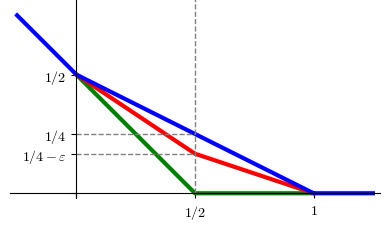
\includegraphics[width=6.6cm,height=4.5cm]{exponent-all-2.png}
\end{equation*}

\definecolor{darkgreen}{rgb}{0.0,0.5,0}
\begin{equation*}
  \text{{\color{blue} Convexity bound}}
  \quad     
  \text{{\color{darkgreen} Lindel\"{o}f hypothesis}}
  \quad
  \text{\alert{Subconvexity}}
\end{equation*}


How about the \emph{nonvanishing problem}?  Suppose given a family
\begin{equation*}
\mathcal{F}_Q = \left\{ \pi : C(\pi, s) \asymp Q \right\}.
\end{equation*}
As $Q \rightarrow \infty$, find $\pi$ such that $L(\pi, \tfrac{1}{2}) \neq 0$?  Then, determine how many of them there are, and also consider subfamilies.

\begin{example}\label{example:cnfg5jz4zo}
  $\GL_1$ twists.  $\mathcal{F}_Q = \left\{ \pi_0 \times \chi \mid\vert \chi \text{ on } F^\times \backslash \mathbb{A}_F^\times, \, C(\chi ) \asymp Q \right\}$.
  \begin{equation*}
    M_1(Q) := \sum_{\pi \in \mathcal{F}_Q } L(\pi, \tfrac{1}{2} ) \neq 0
    \text{ for } Q \rightarrow \infty.
  \end{equation*}
\end{example}

Note that subconvexity improves upon nonvanishing:
\begin{equation*}
  \left\lvert \left\{ \pi : L(\pi, \tfrac{1}{2} ) \neq 0 \right\} \right\rvert
  \gg \frac{\lvert \mathcal{F}_Q  \rvert^{1 + o(1)}}{Q^{1/4 - \delta }}.
\end{equation*}

Another way to get at nonvanishing is to consider also a second moment:
\begin{equation*}
  M_2(Q) := \sum_{\pi \in \mathcal{F}_Q } \lvert L(\pi, \tfrac{1}{2} )  \rvert^2
  = \lvert \mathcal{F}_Q  \rvert^{1 + o(1)}?
\end{equation*}
If one can show this asymptotic, then one deduces
\begin{equation*}
  \left\lvert \left\{ \pi : L(\pi, \tfrac{1}{2} ) \neq 0 \right\} \right\rvert
  = \lvert \mathcal{F}_Q  \rvert^{1 - o(1)}.
\end{equation*}

A basic tool for doing this sort of analysis is the approximate functional equation:
\begin{equation*}
  L(\pi, \tfrac{1}{2} ) = \sum_n \frac{\lambda_\pi(n) }{ n^{1/2} } V \left( \frac{n}{X} \right)
  + \eps(\chi) \sum_n \frac{\overline{\lambda_\pi(n) }}{ n^{1/2} }
  W \left( \frac{n}{Y} \right).
\end{equation*}
Here $X Y = Q$.  One could take, for instance, $X = Y = \sqrt{Q}$; then each sum would have length roughly $\sqrt{Q}$.  One faces in this way
\begin{equation*}
  \sum_{\pi \in \mathcal{F}_Q}
  \lambda_\pi(n),
  \quad
  \sum_{\pi \in \mathcal{F}_Q } \lambda_\pi(m)
  \overline{\lambda_\pi(n)} \eps(\pi)
\end{equation*}
which gives rise to
\begin{equation*}
  \sum_{\chi(q)} \chi(m) \overline{\chi(n)}
  = \varphi(q) \delta_{m \equiv n(q)} 
\end{equation*}
and more generally one gets stuff that one can study using trace formulas.

Another approach is to write $L(\pi, \tfrac{1}{2})$ as an automorphic period and then to use the RTF.

Variant: twisted moments
\begin{equation*}
\sum_\pi L(\pi, \tfrac{1}{2} ) \lambda_\pi(\ell ).
\end{equation*}
This can be useful to single out some $\pi$ inside $\mathcal{F}_Q$.  It can sometimes be used to prove nonvanishing for a \emph{positive proportion} of $\pi$, i.e.,
\begin{equation*}
  \left\lvert \left\{ \pi \in \mathcal{F}_Q  : L(\pi, \tfrac{1}{2} ) \neq 0 \right\} \right\rvert
  \geq c
  \lvert \mathcal{F}_Q \rvert, \quad c > 0.
\end{equation*}
Mollification method:
\begin{equation*}
  \sum L(\pi, \tfrac{1}{2}) m(\pi, L),
  \quad
  m(\pi, L) := \sum_{\ell \leq L}
  \frac{\mu(\ell) \lambda_\pi(\ell)}{\ell^{1/2}}.
\end{equation*}
Here $m(\pi,L)$ is called a \emph{mollifier}.  One takes $L := Q^\alpha$ with $\alpha > 0$ fixed.  It's chosen so that we'll have
\begin{equation*}
  L(\pi, \tfrac{1}{2} ) m(\pi, L) = 1 + \sum_{m \geq L}
  \frac{\lambda_\pi(m)}{m^{1/2}}.
\end{equation*}
This gap in the coefficients is what allows you to get a positive proportion.  (Selberg's work on the positive proportion of zeros of zeta on the critical line.  Iwaniec--Sarnak's paper on nonvanishing.)

Chinta: for $f$ of weight $2$, and $q$ prime,
\begin{equation*}
  \left\lvert \left\{ \chi(q) : L(f \times \chi, \tfrac{1}{2} ) \neq 0 \right\} \right\rvert
  = q - 1 + \O \left( q^{7/8 + \eps} \right).
\end{equation*}
This is a very strong proportion of nonvanishing.  Nothing like this is available for, e.g., Maass forms.

Let's now talk about the subconvexity problem.  This is ostensibly about a single $L$-function, but many proofs of estimates use families.  Suppose we want to show
\begin{equation*}
L(\pi_0, \tfrac{1}{2}  ) \ll C(\pi_0 )^{1/4 - \delta}, \quad \delta > 0.
\end{equation*}
Suppose that $L(\pi_0, \tfrac{1}{2} ) \geq 0$.  For $\pi_0 \in \mathcal{F}_Q$, one expects
\begin{equation*}
  L(\pi_0, \tfrac{1}{2} ) \leq \sum_{\pi \in \mathcal{F}_Q} L(\pi, \tfrac{1}{2} )
\ll \lvert \mathcal{F}_Q  \rvert^{1 + o (1)}.  
\end{equation*}
If $\lvert \mathcal{F}_Q \rvert \leq Q^{1/4 - \delta}$, then one solves the problem.  A spectacular example can be found in the work of Conrey--Iwaniec and Petrow--Young.  They show that for a Dirichlet character $\chi$ of conductor $q$,
\begin{equation*}
L(\chi, \tfrac{1}{2} ) \ll q^{1/6 + o(1)}.
\end{equation*}
In this case, we don't have nonnegativity, so they pass to
\begin{equation*}
  {\left( L(\chi, \tfrac{1}{2} ) L(\bar{\chi}, \tfrac{1}{2} ) \right)}^3
  =
  {L(\chi \boxplus \bar{\chi}, \tfrac{1}{2} )}^3
  = L\left(3 \boxtimes \left( \chi \boxplus \bar{\chi} \right), \tfrac{1}{2} \right).
\end{equation*}
They work with the family
\begin{equation*}
\left\{ 3 \boxtimes(f \times \chi ) : f \in S(q, \bar{\chi}^2) \right\}.
\end{equation*}

It often happens that
\begin{equation*}
\lvert \mathcal{F}_Q  \rvert^{1 + o(1)} = Q^{1/4}.
\end{equation*}
In such cases, \emph{amplification} sometimes works.
\begin{equation*}
  m_{\pi_0}(L) L(\pi_0, \tfrac{1}{2}) \leq \sum L(\pi, \tfrac{1}{2}) m_\pi(L)^2
  \ll \lvert \mathcal{F}_Q  \rvert^{1 + o(1)} = Q^{1/4},
\end{equation*}
\begin{equation*}
  m_\pi(L) := \sum_{\ell \leq L}
  \frac{x_{\ell} \lambda_\pi(\ell)}{\ell^{1/2}},
  \quad
  m_{\pi_0 } \gg L^\alpha , \quad 0 < \alpha \leq 1/2.
\end{equation*}
One takes $L$ to be a small enough power of $Q$.

Now let's talk about an application, returning to the setting of Chris's talk.  Take $B/\mathbb{Q}$ a quaternion algebra.  Take $G = \PB^\times \supset T \cong \Res_{K / \mathbb{Q} } \mathbb{G}_m / \mathbb{G}_m $, and $\chi$ on $T$ of weight zero.  Take $\pi_{\mathrm{JL}}$ on $G$.  Then
\begin{equation*}
  \frac{L(\pi_K \times \chi, \tfrac{1}{2} )}{ C(\pi_K \times \chi)^{1/4}}
  \asymp \left\lvert \int_{[T]} \varphi(t) \chi(t) \, d t \right\rvert^2.
\end{equation*}
How to get something like surjectivity of quotiented-versions of the map $[T] \rightarrow [G]$, as mentioned in Chris's talk?  Average over $\chi$:
\begin{equation*}
  \sum_\chi
  \frac{L(\pi_K \times \chi, \tfrac{1}{2} )}{ C(\pi_K \times \chi)^{1/4}}
  \asymp
  \sum_\chi 
  \left\lvert \int_{[T]} \varphi(t) \chi(t) \, d t \right\rvert^2
  = h_c \int_{[T]} \lvert \varphi \rvert^2
\end{equation*}
by Parseval.  If one can show that $\int_{[T]} \lvert \varphi \rvert^2 > 0$ as $T \rightarrow \infty$, then it will prove that at least one of the $L$-values on the left hand side does not vanish.  One has the equidistribution theorem of Duke, to the effect that $[T] \subset [G]$ is essentially equidistributed.  This means typically that $\int_{[T]} \lvert \varphi \rvert^2$ converges to $\int_{[G]} \lvert \varphi  \rvert^2$, which gives the required nonvanishing.  One can understand this spectrally:
\begin{equation*}
  \int_{[T]} \lvert \varphi  \rvert^2 = \int_{[T]} \sum_\psi \langle \lvert \varphi  \rvert^2, \psi \rangle \psi
\end{equation*}
then use that
\begin{equation*}
 \int_{[T]} \psi(t) \, d t \xrightarrow{?} \int_{[G]} \psi.
\end{equation*}

Vatsal setting:
\begin{equation*}
  \int_T \varphi(t) \bar{\varphi}(t_1 t) \, d t,
\end{equation*}
where $t_1$ is growing a lot with $p^k $, $k \geq 0$.  Here $t_1^h = 1$, where $h = h_K$ is the class number.  Vatsal used homogeneous dynamics, Ratner theory.

We can now obtain similar assertions even when the variation is not vertical, but even when it is more oblique or horizontal.  This uses new analytic techniques and homogeneous dynamics.  Techniques of Holowinsky--Soundararajan, Einsiedler--Lindenstrauss.  One thing this uses is that $\lvert \lambda_\pi(n) \rvert$ is a multiplicative function.

\section{Problem session, moderated by Abhishek Saha}\label{sec:cnfhlpu15t}

\begin{enumerate}
\item\label{enumerate:cnej3fpbu9} (Philippe Michel) Let $f$ be a modular form for $\GL_2$, let $K$ be a quadratic extension, and let $\chi$ be a class group character for $K$.  The Gross--Zagier formula relates
  \begin{equation*}
    L'(f \otimes \theta_\chi, 1)
  \end{equation*}
  to intersection numbers.  The problem is to find a form $g$ be a form on a definite quaternion (perhaps enjoying a congruence with $f$) such that the above $L$-value is directly related to
  \begin{equation*}
    L(g \otimes \theta_K, 1).
  \end{equation*}
  Philippe knows a connection between the two, but it's very loose, and one cannot deduce a lot of nonvanishing in that way.  Use that the Gross--Zagier formula uses in its local term intersection numbers defined using definite quaternion algebras.  (Templier's thesis did something more roundabout.)

\item\label{enumerate:cnej3fpe3c} (Wei Zhang)
  \begin{enumerate}
  \item Given an automorphic representation $\pi$ on $\U(n)$, show that there exists $\sigma$ on $\U(n - 1)$, perhaps in a restricted family, so that $L '(\pi \times \sigma, \tfrac{1}{2})$ is nonzero.  (Maybe even hard if we vary over both $\pi$ and $\sigma$?)
  \item Prove an analogue for algebraic cycles.
  \item (Mladen Dimitrov) Is there any hope to $p$-adically interpolate derivatives?  (Some people suggested the answer ``no''.)
  \end{enumerate}
\item\label{enumerate:cnej3fpha2} (Chris Skinner) Equidistribution of CM points in a single modular curve.  Ilya Khayutin has analogues for joint equidistribution.  How about analogues of Ilya's results, but over a number field $F$?
\item\label{enumerate:cnej3fqemr} Adapt techniques used to estimate automorphic periods to the setting of arithmetic GGP.
\item\label{enumerate:cnej3fqfnd} (Mladen Dimitrov) Take your favorite reductive group $G$ over a $p$-adic local field $F$.  Take an admissible representation $\pi$.  Take a subgroup $H$.  Denote by $K_H(p^n)$ the set of elements in $G(\mathfrak{o})$ that are congruent modulo $p^n$ to something in $H(\mathfrak{o})$.  Then determine whether $\pi$ has vectors fixed under the group $K_H(p^n)$.  Does there exist such an $n$?  And what is the smallest $n$ that works?

  For instance, the case of $H = \GL_{n-1} \times \GL_1$ inside $G = \GL_{n}$ is related to newvector theory (JPSS).  How about more generally $\GL_a \times \GL_b$, possibly for special $\pi$?
\item\label{enumerate:cnej3kgqgj} (Ashey Burungale) Let $p$ be a fixed odd prime.  Consider characters of $(\mathbb{Z} / q)^\times$, where $q$ is a prime.  The question is, how many Dirichlet characters modulo $q$ have the property that $L(0, \chi )$ is $p$-indivisible?  We know $q^{1/2 - \eps}$.
\item\label{enumerate:cnej3kgrc4} (Philippe Michel) Fix an imaginary quadratic field $K$.  We know equidistribution for CM points for order of (squarefree) conductor $C \rightarrow \infty$.  Is there an arithmetic application?  More generally, similar results in broader contexts.
\item\label{enumerate:cnej3kgr45} (Dinakar Ramakrishnan) Given $f$ and a quadratic twist $f \otimes \chi$, can we find a quadratic character $\eta$ so that $f \otimes \eta$ and $f \otimes \chi \eta$ simultaneously have nonvanishing $L$-value?
\item\label{enumerate:cnej3kgsw6} (Ashey Burungale) Another question, along the lines of Philippe's question.  There have been several results toward the Hecke orbit conjecture, which is a mod $p$ analogue of the Andre--Oort conjecture.  There are some results of this nature used by Hida in proving some Iwasawa-theoretic mod $p$ nonvanishing.  Given the progress on the Hecke orbit conjecture, are there potential applications along such lines?
\item\label{enumerate:cnej3kgmi0} Take $\GL_2$ over an imaginary quadratic field.  Consider a Bianchi modular form.  How do you normalize its Whittaker expansion?
\item\label{enumerate:cnej3kglp3} Bocherer's conjecture (now proved in many cases) relates Fourier coefficients of Siegel modular forms to $L$-values.  Let $F$ be a Siegel modular form.  Let $\Lambda$ be a character of the class group $\mathrm{Cl}_d$.  Then
  \begin{equation*}
    \left\lvert \sum_{s \in \mathrm{Cl}_d } a(F, S) \Lambda(S)  \right\rvert^2
    \,\, \dot{=} \,\,
    L(\tfrac{1}{2}, \pi_F \times \theta_\Lambda)
    =
    L(\tfrac{1}{2}, \mathrm{BC}_{K/\mathbb{Q}} \pi_F \times \Lambda).
  \end{equation*}
  If we know lots of $L$-values (maybe all of them), can we compute the Fourier coefficients?

  More generally, in any GGP setup, if we know all the $L$-values, what can we say about the coefficients, or whatever?
\item\label{enumerate:cnej3mdce1} Given a paramodular newform of weight two with rational coefficients, can you construct the corresponding abelian surface?  \cite{MR3981316}
\item\label{enumerate:cnej3mdbho} In the setting of question \eqref{enumerate:cnej3fqfnd}, when is the space of $K_H(p^n)$-fixed vectors one-dimensional?  Is there always an $H$ for which this happens?  Is there a commonality between such $H$?
\item\label{enumerate:cnej3mc9yo} Let $\pi$ an irreducible admissible infinite-dimensional representation of $\GSp_{2 n}(\mathbb{Q}_p)$.  Set
  \begin{equation*}
    R(n) := \left\{
      g \equiv \diag(1,\dotsc,1,a,\dotsc,a) \pmod{p^n} \text{ for some } a \in \mathbb{Z}_p^\times
    \right\}.
  \end{equation*}
  Does $\pi$ always admit a nonzero vector invariant by $R(n)$?
\item\label{enumerate:cnej3mc563} Coleman: if you have a CM modular form and you take the critical $p$-stabilization, then that lies in the image of the ??? operator.  The question is whether you can do this for a higher-rank group.  Can you find a $p$-adic differential operator and an endoscopic form such that all $p$-stabilizations with respect to the form lie in the image of the operator?

  For example, are the special forms (Yoshida, Saito--Kurokawa) captured by some $p$-adic differential operators?  Generalization of Colmez exact sequence?
\item\label{enumerate:cnej3mcyt4} Prove Beilinson's conjecture for Hecke characters of a quartic CM field.
\item\label{enumerate:cnej3mrs9m} Let $f$ be a weight one cusp form.  Consider the trace-free adjoint representation.  The Harris--Venkatesh conjecture describes the Stark units mod $p$ for this adjoint representation.  Can one develop some sort of local-to-global principle by which, assuming the Harris--Venkatehs conjecture, one can describe Stark units in characteristic zero?

  Are there specific examples where the Stark conjecture is not known?  Say in some exotic cases.
\item\label{enumerate:cnej3m2v7l} Let $F$ be a Siegel cuspidal eigenform, say of full level and weight $k$.  How big are the Fourier coefficients of $F$?  Feel free to assume any standard conjecture, e.g., GRH and all expected period formulas.

  Prove, under this assumption, that
  \begin{equation*}
    \left\lvert a(F, S) \right\rvert \ll_F \det(S)^{\frac{k}{2} - \frac{1}{2} - \delta}
  \end{equation*}
  for some $\delta > 0$.

  Note that, under GRH, the case $\delta = 0$ has been addressed.
\end{enumerate}

\section{Tuesday afternoon organization session}\label{sec:cnfhlpu0zj}

\begin{enumerate}
\item\label{enumerate:cnekjr1oym} Tighten connections between $L'(\pi_K \otimes \chi, \tfrac{1}{2} ) \neq 0$ and $L(\sigma_K \otimes \chi ', \tfrac{1}{2} ) \neq 0$.
\item\label{enumerate:cnekjr1pna} Applications of results for horizontal variation of $\chi$ and $\chi '$.
\item\label{enumerate:cnekjr1p68} Given $\varphi \in \pi $ for $\U(n, 1)$ (and maybe it corresponds to something holomorphic, so that what is happening at $\infty$ is fixed), find $\sigma$ and $\psi \in \sigma$ for $\U(n)$ such that the period does not vanish, i.e., $\int_{[\U(n)]} \varphi \psi \neq 0$, or maybe that the period is nonzero modulo $p$.
\item\label{enumerate:cnekjr1qyd} Do everything for $L '(\pi \otimes \sigma, \tfrac{1}{2})$ and cycles (AGGP).
\item[4.5]\label{enumerate:cnekjr1s9k} Find examples of \eqref{enumerate:cnekjr1p68} and analogue for cycles.
\item\label{enumerate:cnekjr5mnb} Count the number of odd Dirichlet characters $\chi$ modulo $N$ such that $L(0, \chi )$ is a $p$-adic unit, with varying $N$.
\item\label{enumerate:cnekjr47jp} Invariants in admissible representations under the action of certain open compact subgroups in $G(\mathbb{Z}_p)$.
\item\label{enumerate:cnekjr46s8} $L(f \otimes \chi, \tfrac{1}{2} ) L(g \otimes \chi, \tfrac{1}{2} ) \neq 0$ for some quadratic $\chi$?
\item\label{enumerate:cnekjr5udx} Beilinson's conjecture for the adjoint of a modular form $\ad^0(f) \otimes \chi$, or even a triple product $L$-function $f \otimes g \otimes h$, using the cohomology of $\GSp_4$.
\item\label{enumerate:cnekjr9kus} Relation between Fourier coefficients of Siegel modular forms and $L$-values, assuming something like Bocherer's conjecture.
\item\label{enumerate:cnekjr9lm8} For a definite quaternion algebra $B$ over $F$, and a quadratic subalgebra $K \hookrightarrow B$, try to show that
  \begin{equation*}
    \Pic(K) \rightarrow X_B \times X_B 
  \end{equation*}
  equidistributes as ``$K \rightarrow \infty$''.  (Theorem of Khayutin when $K = \mathbb{Q}$.  Can we generalize it to, say, real quadratic fields.)
\end{enumerate}


\section{Problem sessions}\label{sec:cnfhlpu0ac}
\textbf{Tuesday}.

$L'(\pi \otimes \sigma, \tfrac{1}{2} )$

Analytic.

Given $\pi$ on $[G]$, can you find $\sigma$ on $[H]$ such that $L '(\mathrm{BC}(\pi)\times \mathrm{BC}(\sigma), \tfrac{1}{2} ) \neq 0$?

(Given $\sigma$, can you find $\pi$?)

There's a Jacquet--Rallis trace formula in this setting.

Require that $\pi _\infty$ be cohomological.  Take $\sigma _\infty$ fixed.

Let $K/\mathbb{Q}$ be quadratic.  Take
\begin{equation*}
G' := \GL_n(K) \times \GL_{n - 1}(K),
\end{equation*}
\begin{equation*}
H_1 ' := \GL_{n - 1}(K),
\end{equation*}
\begin{equation*}
H_2 ' := \GL_n(\mathbb{Q}) \times \GL_{n - 1}(\mathbb{Q}),
\end{equation*}
\begin{equation*}
f \in C_c^\infty(G'(\mathbb{A})).
\end{equation*}
Then
\begin{equation*}
  \int \int K_f(h_1', h_2')
  \lvert h_1' \rvert^s
  \eta(h_2')
  \, d h_1' \, d h_2'
  =
  \sum_{
    \substack{
      \pi \boxtimes \sigma  \\
       \text{from unitary}
    }
  }
  L(\pi \boxtimes \sigma, s)
  \times (\dotsb).
\end{equation*}
Take $f = f_n \otimes f_{n - 1}$.

Fix $\sigma_K \ni u$.  Let $x \in \GL_{n - 1}(K_{\mathbb{A}})$ and $y_1 \in \GL_{n - 1}(\mathbb{A}_{\mathbb{Q}})$ and $y_2 \in \GL_n(\mathbb{A}_{\mathbb{Q}})$.

\begin{equation*}
  \int
  \int u(x) \overline{u(y_1)}
  K_{f_n}(x, y_2)
\end{equation*}


\begin{equation*}
\int \int u(x) K_{f_n}(x, y) \lvert x \rvert^s \, d x \, d y.
\end{equation*}

\begin{equation*}
\left( \int_{[\GL_n]} K_f(x, y) \, d y \right) \lvert x \rvert^s \, d x.
\end{equation*}
The inner integral becomes
\begin{equation*}
K_{\tilde{f}}(\dotsb).
\end{equation*}

\begin{equation*}
S_n = 
\end{equation*}<++>


\begin{equation*}
I_n(f, s) := \int_{[H_1]} u(x) \lvert x \rvert^s K_{\tilde{f}}(x \cdot 1_n) \, d x.
\end{equation*}
\begin{question}\label{question:cnfg5j0r2o}
  Does there exist $f \in C_c^\infty(G(\mathbb{A}_K))$ such that
  \begin{equation*}
    \frac{d}{d s}
    I_n(f, s)|_{s=0} \neq 0.
  \end{equation*}
\end{question}
Look at the geometric side:
\begin{align*}
  &\int_{[H_1']} u(x) \sum_{\gamma \in G_n(K)} \int f(x^{-1} \cdot \gamma y) \,d y
  \\
  &\quad
    =
    \sum_{G_{n - 1}(K) \backslash G_n(K) / G_n(\mathbb{Q})}
    \int_{G_{n-1}(\mathbb{A}_K) \times G_n(\mathbb{A}_{\mathbb{Q}})} u(x) f(x^{-1} \gamma y) \, d x \, d y.
\end{align*}

If we take $K = \mathbb{Q} \times \mathbb{Q}$, then we're looking at
\begin{equation*}
\int_{[G_n]} \sum_\gamma f(x^{-1} \gamma y).
\end{equation*}
We have $x =(x_1, x_2)$.  We have $f = f_1 \otimes fl2$.  The above becomes
\begin{equation*}
\sum_{\gamma '} K_{f_1 \ast f_2}(x_1^{-1} \gamma ' x_2).
\end{equation*}
The question becomes whether
\begin{equation*}
0 \neq \int_{G_{n - 1}(\mathbb{A}_K)} u(x) K_{\tilde{f}}(x) \,d x.
\end{equation*}
Here $K_{\tilde{f}}$ is right-invariant under $G_n(\mathbb{A}_{\mathbb{Q}})$, left-invariant under $G_n(K)$.

Let us now insert the Whittaker expansion of $u$.

We have
\begin{align*}
  W(x) &= \sum_{\delta \in N_{n - 2}(K) \backslash G_{n - 2}(K)} W(\delta x) \\
       &= \sum_{\delta \in N_{n - 1}(K) \backslash P_{n - 1}(K)} W(\delta x).
\end{align*}
Unfolding, and paying attention only to the trivial coset for $P_{n-1}(K) \backslash G_{n-1}(K)$, we arrive at
\begin{equation*}
  \int_{N_{n - 1}(K) \backslash G_{n - 1}(\mathbb{A}_K)}
  W(x) K_{\tilde{f}}(x),
\end{equation*}
\begin{equation*}
K_{\tilde{f}}(x) = \sum_{\gamma \in S_n(\mathbb{Q})} \tilde{f}(x^{-1} \cdot \gamma).
\end{equation*}
We arrive at
\begin{equation*}
  \sum_{\gamma \in N_{n - 1}(K) \backslash S_n(\mathbb{Q})}
  \int_{G_{n - 1}(\mathbb{A}_K) / \mathrm{Stab}}
  W(x) \tilde{f}(x^{-1} \cdot \gamma) \, d x.
\end{equation*}

Something like
\begin{equation*}
\int_{G_{n - 1}(\mathbb{A}_K) / N_{n - 1}(\mathbb{A}_{\mathbb{Q}})} W(x) \tilde{f}(x) \, d x.
\end{equation*}
This is something like $W(1)$.

What is the moment we're considering?  We're looking at
\begin{equation*}
  \sum_{\pi } L(\pi \otimes \sigma, s)
\end{equation*}
where $\sigma$ is fixed on $G_{n-1}(K)$ and $\pi$ is varying over $G_n(\mathbb{Q})$-distinguished automorphic things on $G_n(K)$.

So this would be like
\begin{equation*}
  \sum_{\pi \text{ on } G_n(\mathbb{Q})}
  \lvert L(\pi \sigma, s ) \rvert^2.
\end{equation*}


AGGP conjecture.

Let $K /\mathbb{Q}$ be imaginary quadratic.  Let $W \subseteq V$ with signatures $(1, n - 2)$ and $(1, n - 1)$.

$\mathrm{Sh}(W) \hookrightarrow \mathrm{Sh}(V)$,
\begin{equation*}
  Z := \mathrm{Sh}(W) \hookrightarrow \mathrm{Sh}(W) \times \mathrm{Sh}(V) =: X.
\end{equation*}
Hecke translation
\begin{equation*}
\left\langle R(f) Z, Z \right\rangle_{\height} = \sum_{\pi, \sigma} L '(\tfrac{1}{2}, \pi_K \times \sigma_K ) \times (\text{local terms}).
\end{equation*}

\begin{equation*}
\langle R(f) Z, Z \rangle_{\height} = \sum_p \left\langle R(f) Z , Z \right\rangle_p.
\end{equation*}

\begin{equation*}
I(f) = \sum_{\gamma \in B(F)} I_\gamma(f),
\end{equation*}
where
\begin{equation*}
B = H_1 ' \backslash G ' / H_2 '.
\end{equation*}

\begin{equation*}
K_{f, 1}(x, y) = \sum_{\gamma \in G_1 '(\mathbb{Q})} f(x^{-1} \gamma y),
\end{equation*}
\begin{equation*}
I_1^T(f) := \int (K_{f, 1}(x, y) + \text{error term}) \eta(y) \, d y.
\end{equation*}


\textbf{Wednesday}.

Let $K / \mathbb{Q}$ be a quadratic extension.  Set
\begin{equation*}
  G ' := \GL_{n, K} \times \GL_{n - 1, K}.
\end{equation*}
It contains the subgroups
\begin{equation*}
  H_1 ' := \GL_{n - 1, K}, \qquad H_2 ' := \GL_{n, \mathbb{Q}} \times \GL_{n - 1, \mathbb{Q}}.
\end{equation*}
Let
\begin{equation*}
  f \in C_c^\infty(G '(\mathbb{A})).
\end{equation*}
We consider the integral
\begin{equation*}
  I(f, s ) = \int_{[H_1 ' ] \times [H_2 ' ] } K_f(h_1, h_2 ) \lvert h_1  \rvert^s \eta(h_2 ) \, d h_1 \, d h_2.
\end{equation*}
It admits the geometric expansion
\begin{equation*}
  I(f, s) = \sum_{\gamma \in B(\mathbb{Q} )} I_\gamma(f , s).
\end{equation*}
Here $B$ is the GIT quotient
\begin{equation*}
  B := H_1 ' \backslash G ' / H_2 '.
\end{equation*}
It is an affine space of dimension $n$.

At first we localize this: we only want one term here.

For each $f$, there exists a modification $f'$ (obtained by modifying at some given place, e.g., an archimedean place)

\begin{equation*}
  f_1(g_f g _\infty) = f(g_f, g _\infty) u(g _\infty ), \quad u \in C^\infty(G '(\mathbb{R})).
\end{equation*}

We have the quotient map
\begin{equation*}
  q : G \rightarrow B.
\end{equation*}
The fiber $q^{-1}(1)$ contains many cosets, but there are only two \emph{regular} cosets in that fiber.  Call these $\reg^+$ and $\reg^-$.

\begin{remark}\label{remark:cnfg5j17xi}
  What happens in the split case, here?  We would then be looking at something like $\GL_{n-1} \backslash \GL_n$, right?
\end{remark}


Suppose that there exists $v$ such that
\begin{equation*}
  \supp(f_v) \subset \reg^+(\mathbb{Q}_v) \subset^o G '(\mathbb{Q}_v).
\end{equation*}
Then the integral
\begin{equation*}
  I_1^{\mathrm{Tate}}(f, s) = \int_{[H_1'] \times [H_2']}
  K_{f,1}(h_1, h_2) \lvert h_1 \rvert^s \eta(h_2) \, d h_1 \, d h_2
\end{equation*}
converges absolutely when $\Re(s) < -1$ and admits a meromorphic continuation.  The value $0$ (after meromorphic continuation) is what we want:
\begin{equation*}
  I_1^{\mathrm{Tate}}(f, 0) = I_1(f, 0).
\end{equation*}
The Tate regularization gives the same result as the truncation procedure (as in the works of Zydor and Chaudouard et al.).

If we assume a support condition instead with respect to $\reg^-(\mathbb{Q}_v)$, then the analogous integral converges absolutely for $\Re(s) > 1$ and again admits a meromorphic continuation, with similar conclusions.

We have a factorization
\begin{equation*}
  I_1^{\mathrm{Tate}}(f, s) = \prod_v \int_{H_1(\mathbb{Q} ) \times H_2(\mathbb{Q})} f(h_{1, v}^{-1} \gamma_T h_{2, v}) \lvert h_{1, v} \rvert^s \eta(h_{2, v}) \, d h_{1, v} \, d h_{2, v}.
\end{equation*}
At almost every place $v$, the local integral evaluates to $\prod L_{v , j}(s, \chi_i)$.

The upshot is that if we take the support of $f$ small enough at some place, then we only get one term in the whole expansion.

\begin{remark}\label{remark:cnfg5j2du3}
  Let $\pi$ be a representation of $\GL_n \times \GL_{n + 1}$.  Let $\varphi$ be a matrix coefficient of $\pi$, say
  \begin{equation*}
    \varphi(g) = \langle \pi(g) v, v' \rangle.
  \end{equation*}
  Assume for simplicity that $\pi$ is supercuspidal.  Then the relative character may be represented as the orbital integral attached to a matrix coefficient
  \begin{equation*}
    \theta_\pi^H(g) = c_\varphi \operatorname{Orb}(g, \varphi).
  \end{equation*}
  Here
  \begin{equation*}
    \operatorname{Orb}(g, \varphi) = \iint_{H(\mathbb{Q})^2} \varphi(h_1  g h_2) \, d h_1 \, d h_2.
  \end{equation*}
  This is proved in an appendix of Wei Zhang and Atsushi Ichino.
\end{remark}

\begin{equation*}
  \prod_{k = 1 }^n L(
  \eta^{-k},
  - k s - k + 1
  ).
\end{equation*}

\begin{example}\label{example:cnfg5j2iii}
  If $n = 1$, then we get
  \begin{equation*}
    L(\eta^{-1}, - s).
  \end{equation*}
\end{example}
\begin{example}\label{example:cnfg5j2kbr}
  If $n =2$, then we get
  \begin{equation*}
    L(\eta^{-1}, - s) L(\eta^{-2}, - 2 s -1).
  \end{equation*}
\end{example}
\begin{example}\label{example:cnfg5j2k8u}
  If $n=3$, then we get
  \begin{equation*}
    L(\eta^{-1}, - s) L(\eta^{-2}, - 2 s -1) L(\eta^{-2}, - 3 s - 2).
  \end{equation*}
\end{example}

Liyang.

Notation: $K/\mathbb{Q}$, $G = \GL_3$, $H = \GL_2$, $\sigma \in \mathcal{A}_0(H(\mathbb{A}_K))$, $\sigma \leftrightarrow \operatorname{BC}(\sigma_0)$.

\textbf{Goal.}
\begin{equation*}
  \sum_{\pi \in \mathcal{A}_0(G(\mathbb{A}_K ))_N}
  L(\tfrac{1}{2} + s, \pi \times \sigma)
  \mathcal{P}_{\pi, \sigma }(f)
  = \mathcal{M}(s) + \mathcal{E}(s).
\end{equation*}
$\frac{d}{d s}$.

\begin{equation*}
  \sum_{\pi = \operatorname{BC}(\pi ')}
  L(\tfrac{1}{2}, \pi \times \sigma)
  \mathcal{P}_{\pi, \sigma}(f) = \mathcal{M} '(0) + 0.
\end{equation*}
The main term should be essentially
\begin{equation*}
  \mathcal{M}(s) \, \dot{=} \, L(1 + s, \sigma, \mathrm{Asai})
  + L(s, \sigma, \mathrm{Asai}).
\end{equation*}
Today we'll focus on the first term on the left hand side.

$f = \otimes_v f_v$, where $f_v \in C_c^\infty(K_v \backslash G_v / K_v)$.

For $v \mid N$, take $f_v = \frac{1}{\vol} \mathbf{1}_{K_v [N]}$.

\textbf{Idea.}
\begin{equation*}
  \int_{[H]}
  \int_{[G]}
  K \left(
    \begin{pmatrix}
      x      &  \\
             & 1 \\
    \end{pmatrix}, y \right)
  \phi(x) \, d y \,d x.
\end{equation*}
Here $[G] = \bar{G}(\mathbb{Q}) \backslash \bar{G}(\mathbb{A})$.

The spectral side will be as above.

The geometric side will be
\begin{equation*}
  \int_{[H]} \int_{[G]}
  \sum_{\gamma \in G(K)} f \left(
    \begin{pmatrix}
      x^{-1}       &  \\
                   & 1 \\
    \end{pmatrix} \gamma y \right)
  \phi(x) \, d y \,d x.
\end{equation*}
The orbital integral attached to $1$ evaluates to
\begin{equation*}
  \int_{H(\mathbb{Q}) \backslash H(\mathbb{A}_K)} \int_{\bar{G}(\mathbb{A})} f \left(
    \begin{pmatrix}
      x^{-1}       &  \\
                   & 1 \\
    \end{pmatrix}
    y
  \right)
  \phi(x) \,d y \,d x.
\end{equation*}
Due to the support conditions on $f$, we can write
\begin{equation*}
  y \in
  \begin{pmatrix}
    x    &  \\
         & 1 \\
  \end{pmatrix} K.
\end{equation*}
We then see that the main term is essentially
\begin{equation*}
  \int_{H(\mathbb{Q}) \backslash H(\mathbb{A})} \phi(x) \,d x.
\end{equation*}

We consider the action
\begin{equation*}
  B(K) \backslash G(K) \circlearrowleft G(\mathbb{Q}).
\end{equation*}
This leads to
\begin{align*}
  G(K) &= B(K) G(\mathbb{Q}) \sqcup B(K)
         \begin{pmatrix}
    1    &  &  \\
    \tau & 1 &  \\
         &  & 1 \\
  \end{pmatrix}
         G(\mathbb{Q}) \\
       &\quad \sqcup
         B
         \begin{pmatrix}
           1           &  &  \\
                       & 1 &  \\
                       & \tau & 1 \\
         \end{pmatrix}
         G(\mathbb{Q})
         \sqcup
         B(K)
         \begin{pmatrix}
           1           &  &  \\
                       & 1 &  \\
           \tau &  & 1 \\
         \end{pmatrix} G(\mathbb{Q}).
\end{align*}
This leads to
\begin{equation*}
  \int_{[H]} \int_{[G]_{\mathbb{Q}}}
  K \left(
    \begin{pmatrix}
      x      &  \\
             & 1 \\
    \end{pmatrix}
    , y\right) \phi(x) \lvert x \rvert^s \, d x \,d y.
\end{equation*}
One of the main sources of divergence comes from the degenerate parts of Eisenstein series.  So we need to kill that Eisenstein stuff.

To do that, we consider the Fourier expansion.  Etc.  We get
\begin{equation*}
  \int_{[H]}
  \int_{[G]_{\mathbb{Q}}}
  \sum_{\alpha \in N_H(K) \backslash H(K) }
  K \left(
    u \alpha 
    \begin{pmatrix}
      x      &  \\
             & 1 \\
    \end{pmatrix}
    , y\right)
  \theta(u) \, d u
  \, \phi(x) \lvert x \rvert^s \, d x \,d y.
\end{equation*}
The geometric side now becomes
\begin{equation*}
  \int_{[H]} \int_{[G]_{\mathbb{Q}}} \sum_\alpha
  \int_{[N]}
  \sum_\gamma f \left(
    \begin{pmatrix}
      x^{-1}      &  \\
                  & 1 \\
    \end{pmatrix} \alpha^{-1} u^{-1} \gamma y \right)
  \theta(u) \phi(x) \lvert x \rvert^s \,d x \,d y \,d u.
\end{equation*}
This evaluates to
\begin{equation*}
  \int_{H(\mathbb{Q}) \backslash H(\mathbb{A}_K)}
  \int_{[G]_{\mathbb{Q}}}
  \int_{[N]}
  \sum_\gamma
  f \left(
    \begin{pmatrix}
      x^{-1}      &  \\
                  & 1 \\
    \end{pmatrix} \alpha^{-1} u^{-1} \gamma y \right)
  \theta(u) \phi(x) \lvert x \rvert^s \,d x \,d y \,d u.
\end{equation*}
Now, use that
\begin{equation*}
  \begin{pmatrix}
    1    & \ast & \ast \\
             & 1 & \ast \\
             &  & 1 \\
  \end{pmatrix}
  \cong
  \begin{pmatrix}
    1    & \ast &  \\
         & 1 &  \\
         &  & 1 \\
  \end{pmatrix}
  \begin{pmatrix}
    1    &  & \ast \\
         & 1 & \ast \\
         &  & 1 \\
  \end{pmatrix}.
\end{equation*}
This gives that the above is
\begin{equation*}
  \int_{N(\mathbb{A}_K) \backslash H(\mathbb{A}_K)}
  \int_{[G]_{\mathbb{Q}}}
  \int_{[N]}
  \sum_\gamma
  f \left(
    \begin{pmatrix}
      x^{-1}      &  \\
                  & 1 \\
    \end{pmatrix}
    u^{-1} \gamma y\right)  
  \theta(u) \,d u
  \, W_\phi(x) \,d x \,d y.
\end{equation*}
Look at
\begin{equation*}
  L(1 + s, \sigma, \mathrm{Asai}).
\end{equation*}
Roughly,
\begin{equation*}
  L(s, \sigma, \mathrm{Asai}) = \prod \int_{N(\mathbb{Q}_p) \backslash H(\mathbb{Q}_p)} W(x) \Phi(x) \lvert x \rvert^s_p \,d x_p.
\end{equation*}
We have
\begin{equation*}
  \begin{pmatrix}
    x^{-1}    &  \\
              & 1 \\
  \end{pmatrix}
  \begin{pmatrix}
    1    &  & \ast \\
         & 1 & \ast \\
         &  & 1 \\
  \end{pmatrix}
  \begin{pmatrix}
    x    &  \\
         & 1 \\
  \end{pmatrix}
  =
  \begin{pmatrix}
    1    &  & \ast \\
         & 1 & \ast \\
         &  & 1 \\
  \end{pmatrix}.
\end{equation*}
There's also a modular character.

Get
\begin{equation*}
  \int_{N_p(\mathbb{A}_K)} f \left( u
    \begin{pmatrix}
      x^{-1}      &  \\
                  & 1 \\
    \end{pmatrix} \gamma y \right)
  \theta(\eta x u) \,d u.  
\end{equation*}



\textbf{Thursday.}
\textbf{Wei.}

Let $u : [H] \rightarrow \mathbb{C}$, $H \subset G$.

Then
\begin{equation*}
K_f(x, y) = \sum_{\gamma \in G(\mathbb{Q})} f(x^{-1} \gamma y), \quad f \in C_c^\infty(G(\mathbb{A})).
\end{equation*}

We were looking at
\begin{equation}\label{eq:cnfg56vjen}
\iint_{[H]^2} u(x) u(y) K_f(x, y) \, d x \, d y.
\end{equation}

Now consider
\begin{equation*}
H = \GL_2
\end{equation*}
and
\begin{equation*}
u : X \rightarrow A
\end{equation*}
and
\begin{equation*}
G = \GL_2 \times \GL_2,
\end{equation*}
with $H$ embedded diagonally, and
\begin{equation*}
f \in \mathcal{H}_G = C_c^\infty(G(\mathbb{A}_f)).
\end{equation*}
Then we consider a diagram where $T_f$ has two maps to $S_G = X \times X$.

Then we consider the map
\begin{equation*}
X \xrightarrow{(u, \iota)} A \times S_G = A \times X \times X.
\end{equation*}
Abbreviate $\varphi :=(u, \iota)$.  Then the intersection number
\begin{equation}\label{eq:cnfg58ajpb}
\left\langle \varphi _\ast(X), T_f \ast \varphi _\ast(X) \right\rangle
\end{equation}
is the analogue of \eqref{eq:cnfg56vjen}.  We can write this as a sum of orbital integrals after ``averaging over $\varphi$'':
\begin{equation*}
\sum_v \sum_\gamma \operatorname{Orb}(\gamma, f^\vee) \mathrm{wt}_v(\gamma).
\end{equation*}
Question: can we do so without ``averaging''?

Possibly we can think of \eqref{eq:cnfg58ajpb} more symmetrically as the number we get from considering
\begin{equation*}
  X \times X \xrightarrow{(u,u,\iota,\iota)}
  A \times A \times S_G \times S_G
\end{equation*}
by pushing forward and then pairing against the embedding of $\Delta A \times T_f$.

\textbf{Weixiao.}

Issue.  Suppose that $I'(f, s) \neq 0$.  We claim that we have
\begin{equation*}
I_\pi '(f, s) \neq 0
\end{equation*}
for some cuspidal $\pi$ with $\eps(\pi) = -1$ (so that $L(\tfrac{1}{2}, \pi) = 0$).  We have
\begin{equation*}
  I_\pi '(f, s) =
  \left( L(\tfrac{1}{2} + s, \pi )
  \times (\text{local factors}) \right)'.
\end{equation*}
We have a comparison
\begin{equation}\label{eq:cnfg6c4p6o}
  I_\pi(f') = \sum_{V} \sum_{\sigma \in \mathcal{A}_{\cusp}(\U(V) \times \U(V \oplus E))}
  J_\sigma(f),
\end{equation}
where $f ' = \otimes f_v '$ and $f = \otimes f_v$ correspond under smooth transfer:
\begin{equation*}
\operatorname{Orb}(\gamma, f_v ') = \operatorname{Orb}(\delta, f_v),
\end{equation*}
for regular semisimple $\gamma \leftrightarrow \delta$.

A function $f_v'$ on the general linear side is transferred to two functions on the unitary side.  We want $f'$  to be of ``pure type'', which means that each $f_v '$ transfers to $\{f_v, 0\}$.  If this happens, then in the sum over $V$ in \eqref{eq:cnfg6c4p6o}, only one term contributes.

We have
\begin{equation*}
I_\pi(f') = J_\sigma(f), \quad \operatorname{BC}(\sigma) = \pi.
\end{equation*}
We have
\begin{equation*}
I_\pi(f') \neq 0 \implies J_\sigma(f) \neq 0 \implies \eps(\pi) = -1,
\end{equation*}
where the last step follows by local GGP.

\begin{proposition}[Wei for $n = 3$, Beuzart-Plessis]
  (local) $I_1^{\mathrm{Tate}}(f') = \eps_1 J_1(f_1) + \eps_2 J_1(f_2)$, where $J_1(f) = \int_{\U(n)} f(h) \, d h$.
\end{proposition}

Say we take $f ' = \otimes f_v '$.  Choose $v_0$ inert, take $f _{v_0}'$ with regular semisimple support, want to arrange that $I_{\pi_{v_0 }}'(f_{v_0 }', 0) = 0$ for all $\pi_{v_0}$.  At $v_1$, we take small support.  Away from those places, maybe we do unramified (or maybe at another place, we do supercuspidal).  Could arrange that $I_{\pi_0 }(f_{v_0 })$ vanishes or not according as $\eps_{v_0}$ is $1$ rather than $-1$.  Arrange that at $v_2$, we take $f_{v_2}$ so that $I_{\pi_{v_2 }}'(f_{v_2}, 0) = 0$.

Suppose that $I_{\pi_{v_0}}(f_{v_0}, s)$ has a functional equation such that it is even provided that $\eps_{\pi_v} = +1$ and odd if $\eps_{\pi_v}$ is $-1$.









\section{Wei Zhang}\label{sec:cnfhlpuzlg}

Cycles vs. $L$-values.

Periods.

$H \subseteq G$ reductive over $F$ global.  $\int_{[H]} \varphi(h) \, d h$, possibly with a weight factor.  $\varphi \in \pi$.  Automorphic representations, possibly tempered, of $G$.  Relate to $L(\pi, \tfrac{1}{2})$ times a product of local terms.  Example: $G = \U(n) \times \U(n-1)$ and $H = \U(n-1)$.

Example: Waldspurger, $G = \GL_2$ or $B^\times $ and $H = \Res_{K / \mathbb{Q}}\mathbb{G}_m$.

$G = \U(n) \times \U(n)$ and $H = \U(n)$.  $\pi_1 \boxtimes \pi_2$.

Also, $\Res_{E / \mathbb{Q}} \U(n)$.

Weil representation of $H =\U(n)$.  $\mu$ : Hecke character with $\mu |_{\mathbb{A}_{\mathbb{Q}}^\times } = \eta_{K/\mathbb{Q}}$.  (Fourier--Jacobi GGP.)

\begin{equation*}
\int_{[H]} \varphi_1(h) \varphi_2(h) \theta_\phi^\mu(h) \, d h.
\end{equation*}
related to
\begin{equation*}
L\left(\mathrm{BC}(\pi_1) \boxtimes \mathrm{BC}(\pi_2) \otimes \mu, \tfrac{1}{2}\right).
\end{equation*}

Friedberg--Jacquet.  $G = \U(2 n) \supseteq H = \U(n) \times \U(n)$.  $\pi$ gives rise to $L(\mathrm{BC}(\pi), \std, \tfrac{1}{2})$.

We turn now to the arithmetic analogue of GGP.

$\pi$ needs to satisfy the analogue of the ``weight two'' condition in the classical setting.  Responsible for cohomology of the Shimura variety.

$G = \U(n - 1, 1) \times \U(n - 2, 1)$.

$H = \U(n-2,1)$.

$\mathrm{Sh}(H) \rightarrow \mathrm{Sh}(G)$.

Dimensions over $\mathbb{C}$: $n - 2$ and $(n - 1) +(n - 2)$.

dimensions over $\mathbb{Z}$: $n - 1$ and $2(n - 1)$.

$\varphi : [G] \rightarrow \mathbb{C}$.

\begin{example}\label{example:cnfg5j3x18}
  Gross--Zagier ($n = 2$).  Let $A$ be an elliptic curve over $\mathbb{Q}$.  Take
  \begin{equation*}
    \varphi : X_0(N) \rightarrow A.
  \end{equation*}
  Then we can make sense of
  \begin{equation*}
    \int_{\mathrm{Sh}(H)} \varphi \in A(K^{\mathrm{ab}}).
  \end{equation*}
  This means to take the pushforward of a divisor.

  Neron--Tate height pairing on the rational points gives an analogue of the metric in the setting of automorphic forms, which allows us to form $\lvert \varphi \rvert^2$.
  \begin{equation*}
    \left\langle
      \int_{\mathrm{Sh}(H)} \varphi,
      \int_{\mathrm{Sh}(H)} \varphi
    \right\rangle_{\mathrm{NT} \text{ height}} = L '(\pi_K, \tfrac{1}{2}).
  \end{equation*}
  For general $n$ and $\pi$,

  we assume that there is some decomposition of the Chow group: $\operatorname{Ch}(\operatorname{Sh}(G)) = \oplus_\pi \operatorname{Ch}(\operatorname{Sh}(G))_\pi$.  Factors through cohomology.
  
  \begin{equation*}
    \left\langle [\mathrm{Sh}_H]_\pi, [\mathrm{Sh}_H]_\pi \right\rangle
    \leftrightarrow
    L '(\pi, \tfrac{1}{2}).
  \end{equation*}

  We can also take $p$-adic heights.
  \begin{equation*}
    \mathrm{Ch}(\mathrm{Sh}_G) \rightarrow  H^1_f(K, H^\ast(\mathrm{Sh})(?))
    = \bigoplus_\pi H_f^1(K, \rho_\pi) \boxtimes \pi_0^\vee.
  \end{equation*}
  Block--Kato Selmer maps(t) the $H^1_f$ factor.

  \begin{theorem}\label{theorem:cnfg5jyfj8}
    \begin{equation*}
      \left\langle \int_{[\mathrm{Sh}(H)]} \varphi, \int_{[\mathrm{Sh}(H)]} \varphi \right\rangle_{\text{$p$-adic height}}
      \approx L_p '(\pi , \tfrac{1}{2}).
    \end{equation*}
    The identity holds up to local factors.
  \end{theorem}

  By comparison, in the setting of automorphic forms, we would be have stuff like
  \begin{equation*}
    \iint_{[H]^2 } u(x) u(y) K_f(x,y) \, d x \, d y.
  \end{equation*}

  
\end{example}

Periods and cycles.
k
aRTF.  $f \in C_c^\infty(G(\mathbb{A}))$.  Can consider
\begin{equation*}
  \iint_{[H]^2 }
  K_f(x, y) \, d x \, d y,
\end{equation*}
which admits expansions
\begin{equation*}
  \sum_{\varphi \in \mathcal{B}(\pi)} \int_{[H]} \overline{\varphi (h)} \int_{[H]} \pi(f) \varphi(h) \, d h
  = \sum_{\gamma \in H \backslash G(\mathbb{Q}) / H(\mathbb{Q}) \operatorname{Orb}(\gamma f).}
\end{equation*}

For $f \in C_c^\infty(G(\mathbb{A}_f))$, look at

\begin{equation*}
  \sum_{v \nmid 0}^{\sharp} + \sum_v \sum_{\gamma \in G^{(v) }} \operatorname{Orb}(\gamma, f^{(v)})
  \partial \operatorname{Orb}(\gamma \cdot f_v ) \log q_v.
\end{equation*}

Let's change the topic to \emph{vanishing}.  In the unitary GGP setting, does there exist an $L$-function with $\ord L(\pi, s) \geq 3$?  ($\eps(\pi) = - 1$, $L '(\pi, \tfrac{1}{2} ) = 0$, $\pi : \GL_2/_F$ totally real.

Qiu:
\begin{equation*}
\ord L(\pi_1 \times \pi_2 \times \pi_3, \tfrac{1}{2}) \geq 3?
\end{equation*}

\section{Ashay Burungale}\label{sec:cnfhlpuyt9}

\subsection{Introduction}\label{sec:cnfhlpux35}
$\mathcal{M}_{/ \mathbb{Q}}$, $L(\mathcal{M}, s)$ critical at $s = 0$. $L^{(r)}(\mathcal{M}, 0)$: Block--Kato, Selmber group.

\begin{question}\label{question:cnfg5j4o4z}
  How often do we have
  \begin{equation*}
    L(\mathcal{M} \otimes \chi, 0) \neq 0
  \end{equation*}
  as $\chi$ varies?
\end{question}
\begin{enumerate}[(i)]
\item The conductor of $\chi$ is a varying prime.
\item The conductor of $\chi$ is a power of a fixed prime.
\end{enumerate}

Iwasawa theory.  Ferrero--Washington, Hida, Vatsal, Finis: mod $p$ non-vanishing.

An ingredient in the proof of $\GL_2$ Iwasawa main conjecture, Skinner--Urban.

Mod $p$ horizontal non-vanishing?

\subsection{Dirichlet L-values}\label{sec:cnfhlpuw9d}
Let $\lambda$: Dirichlet character of conductor $N$.

$\chi$: Dirichlet character of conductor $F$.

$p \nmid 2 F N$ $L(0, \lambda \chi)$ $p$-integral.

$v_p$: $p$-adic valuation.

Set
\begin{equation*}
\mathfrak{X}_\lambda(F) := \left\{ \chi \in \widehat{(\mathbb{Z} / F)^\times } : v_p \left( L(\lambda \chi, 0) \right) = 0 \right\}.
\end{equation*}
In words, this is the set of characters for which the $p$-valuation of the value at $0$ of the Dirichlet $L$-function attached to $\lambda \chi$

\begin{question}\label{question:cnfg5j4tbm}
  How big is $\mathfrak{X}_\lambda(F) $ as a function of $F$?
\end{question}

Ferrero--Washington: $F_n = \ell^n$, $\# \mathfrak{X}_\lambda(F_n) \sim \varphi(\ell^n)$.

As $F$ varies over primes, $\mathfrak{X}_\lambda(F) \asymp F$.

\begin{theorem}[Sun--B]\label{theorem:cnfg5jyjlh}
  Let $F$ be a prime, $p \nmid 2 \varphi(F) F N$.
  \begin{enumerate}[(a)]
  \item\label{enumerate:cnekzumaui} If $F > N$, then
    \begin{equation*}
      \# \mathfrak{X}_\lambda(F) \geq
      \left\lfloor
        \frac{2 [\mathbb{F}_p(\lambda, \zeta_F ) \cdot \mathbb{F}_p(\lambda) ]}{N}
      \right\rfloor^{1/4}.
    \end{equation*}
  \item\label{enumerate:cnekzumb90} If $F > N$, then
    \begin{equation*}
      \# \mathfrak{X}_\lambda(F) \geq
      \left\lfloor
        \left( \frac{F}{9 N} \right)^{1/2}
      \right\rfloor.
    \end{equation*}
  \end{enumerate}
\end{theorem}

\begin{remark}\label{remark:cnfg5j4wud}
  Some examples where $\# \mathfrak{X}_\lambda(F) \sim F$.
\end{remark}

\textbf{Strategy.}

\begin{equation*}
  R_\lambda(r, F) = \sum_{
    \substack{
      \chi \in \widehat{(\mathbb{Z} / F)^\times }  \\
      r \in(\mathbb{Z} / F)^\times, \\
      c(\chi) \in \overline{\mathbb{Z} }_{(p)}
    }
  }
  \chi(r) c(\chi ) L(\lambda \chi, 0).
\end{equation*}

\begin{fact}
  If there exist $\underline{r} =(r_i )$ and $\underline{s} =(s_j )$ in $(\mathbb{Z} / F)^\times$ such that for some $Q$, we have that
  \begin{equation*}
    \det \left( R_\lambda(r_i s_j , F) _{ 1 \leq i, j \leq Q} \right) \not \equiv 0 \pod{p},
  \end{equation*}
  then $\# \mathfrak{X}_\lambda(F) \geq Q$.
\end{fact}

Algebraic approach.

\begin{equation*}
  \Phi_\lambda(T) =
  \frac{\left(
    \sum_{r = 1 }^{N - 1}
  \lambda(r) T^r \right)}{1 - T^N},
\end{equation*}
\begin{equation*}
R_\lambda(r, F) = - \varphi(F) \lambda(- 1) \Phi_\lambda(\zeta_F^r).
\end{equation*}

\textbf{Aim.}  To find $Q$, $\underline{r}$, $\underline{s}$ such that
\begin{equation*}
  \det \left( \Phi_\lambda(\zeta_F^{r_i s_j }) \right) \neq 0 \pod{p}.
\end{equation*}
Put
\begin{equation*}
  D_\lambda(\underline{r}, \underline{s}, T)
  = \sum_{\sigma \in S_{\lvert Q \rvert}}
  \sgn(\sigma) \prod \psi_\lambda(T^{r_1 s_{\sigma(1)}})
  \prod \left( 1 - T^{N r_i s_j} \right).
\end{equation*}
We think of this as an element of $\mathbb{F}_p(\lambda) [T]$.

Let $Q_\lambda(F, T)$ denote the irreducible polynomial of $\zeta_F$ over $\mathbb{F}_p(\lambda)$.

Then it suffices to show that $D_\lambda(\underline{r}, \underline{s}, T) \not \equiv 0 \pod{Q_\lambda(F, T)}$.

This is okay if $\deg D_\lambda < \deg Q_\lambda$.

$\deg D_\lambda \leq N Q^4/2$.

Homological approach.

$R_\lambda(r, F) =(F - 1) \lambda(F) \tau(\lambda) \int_{r/F - i \infty}^{r/F + i \infty} \Phi_\lambda \left( e^{2 \pi i z} \right) \, d z$.

$c(\chi) = \bar{\chi}(N)$.

\begin{equation*}
  I(\lambda, x) = \int_{x - i \infty}^{x + i \infty}
  \Phi_\lambda(e^{2 \pi i z}) \, d z
  \quad \text{ for } x \in \mathbb{R} - \frac{\mathbb{Z}}{N} \pmod{1}.
\end{equation*}

\textbf{Want.} $\underline{r}$, $\underline{s}$,
\begin{equation*}
\det I \left( \lambda, \frac{r_i s_j}{F} \right) \neq 0 \pod{p}.
\end{equation*}

$I(\lambda, x)$: $p$-integral.

$I(\lambda, x) = I(\lambda, y)$ if $\frac{m - 1}{N} \leq x, y \leq \frac{m}{N}$.

$I(\lambda, x) - I(\lambda, y) \neq 0$ if $\frac{m - 1}{N} \leq x < \frac{m}{N} < y \leq \frac{m + 1}{N}$.

\textbf{Reduces to the following.}
$N = 2$.  \textbf{Want}: $\underline{r}, \underline{s}, \underline{s'}$ such that
\begin{enumerate}
\item[$C_1$] $0 < \frac{r_j s_j(F) }{F} < \frac{1}{2} < \frac{r_i s_j '(F) }{F}$ for $1 \leq j \leq Q$.
\item[$C_2$] $0 < \frac{r_j s_j(F) }{F}, \frac{r_i s_j '(F) }{F} < \frac{1}{2}$ for $1 \leq j < i < Q$.
\end{enumerate}

\begin{remark}\label{remark:cnfg5j6hsm}
  It seems from numerics that $Q \asymp F$, but we can only do $Q \asymp F^{1/2}$.
\end{remark}

\subsection{Rankin--Selberg L-values}\label{sec:cnfhlpuwet}
Start with an elliptic curve $E_{/\mathbb{Q}}$.  Let $N_E$ denote the conductor.

Let $K/\mathbb{Q}$ be an imaginary quadratic field with $(D_K, N_E) = 1$.

Let $\chi \in \mathrm{Cl}_K$ denote an ideal class character.

Consider the Rankin--Selberg convolution $L(E \times \chi, s)$, self-dual: $\eps(E_{/K}) = \pm 1$.

The following question was raised in a paper of Michel--Venkatesh.
\begin{question}\label{question:cnfg5j6lyt}
  How often are these central $L$-values $L(E \times \chi, 1)$ nonvanishing, for $\chi \in \widehat{\mathrm{Cl}_K}$ as $K$ varies?
\end{question}

Michel--Venkatesh:
\begin{equation*}
  \# \left\{ \chi \in \widehat{\mathrm{Cl}_K}
    :
    L(E \times \chi, 1) \neq 0
  \right\}
  \gg D_K^\delta \quad \text{ for } 0 < \delta < \frac{1}{2700}.
\end{equation*}

\begin{question}\label{question:cnfg5j6qpg}
  How about
\begin{equation*}
  \# \left\{ \chi \in \widehat{\mathrm{Cl}_K} : v_P \left( L^{\mathrm{alg}}(E \times \chi, 1) \right) = 0 \right\}?
\end{equation*}
\end{question}
\begin{theorem}[Hida--Tian--B]\label{theorem:cnfg5jyk55}
  Suppose that $p \nmid 6 N_E \prod_{\ell \div N} c_{\ell}$ and $\overline{\rho_{E, p}}$ is absolutely irreducible.  Then
  \begin{equation*}
    \# \left\{ \chi \in \widehat{\mathrm{Cl}_K} : v_P \left( L^{\mathrm{alg}}(E \times \chi, 1) \right) \right\}
    \gg \left( \log \lvert D_K \rvert \right)^{1 - \eps}
  \end{equation*}
  as $K$ varies with
  \begin{itemize}
  \item $p \nmid h_K$,
  \item $\eps(E_{/K}) = +1$.
  \end{itemize}
\end{theorem}

\begin{remark}\label{remark:cnfg5j6ys8}
  \begin{itemize}
  \item Proven via $p$-indivisibility of a toric period.
  \item Simultaneously prove result for Tate--Shafarevich groups.
  \end{itemize}
\end{remark}

\textbf{Sketch.}  We have
\begin{equation*}
  L^{\mathrm{alg}}(E \times \chi, 1) = P_\chi(f)^2 c_\chi
\end{equation*}
for
\begin{equation*}
  P_\chi(f) = \int_{B^\times \backslash B^\times_{\mathbb{A}}} \chi(t) f(t) \, d t.
\end{equation*}
Let $B$ be a definite quaternion algebra, and $X_U$ the associated Shimura set.  Let $K \hookrightarrow B$.  Let $\varphi_U : \mathrm{Cl}_K \rightarrow X_U$.

\textbf{Existence of one twist.}  We can arrange that $f \not \equiv 0 \pod{p}$.

If $P_\chi(f) \equiv 0 \pod{p}$ for all $\chi \in \widehat{\mathrm{Cl}_K}$, then
\begin{equation*}
  f \equiv 0 \pod{p} \quad \text{on } \mathrm{Cl}_K.
\end{equation*}

\textbf{Equidistribution}. $\varphi_U(\mathrm{Cl}_K) \twoheadrightarrow X_U$ for $\operatorname{disc}(K) \gg 0$.

It follows that
\begin{equation*}
  f \equiv 0 \pod{p}\quad \text{on } X_U.
\end{equation*}

$\varphi_U(H_K)$ for $H_K \leq \mathrm{Cl}_K$, $[\mathrm{Cl}_K : H_K] \leq D_K^{\delta '}$.

\section{Andrei Jorza}\label{sec:cnfhlpuvgp}
Let's talk about vanishing of $L(\pi, \tfrac{1}{2})$ and $L(\pi \chi, \tfrac{1}{2})$.

There is a dichotomy according as $C(\chi) = p^m$ (Iwasawa) or $C(\chi) = \ell$ (a prime tending off to $\infty$).

Let $f$ be a modular form of weight two that is ordinary at $p$.  Let $\chi$ have conductor $p^m$.  Then
\begin{equation*}
  L_p(f, \chi) = \frac{L(f, \chi, 1)}{\Omega_f^{\pm}}
  \times(\text{extra factors}).
\end{equation*}
If there exists $\chi$ such that $L_p(f, \chi) \neq 0$, then only finitely many $\chi$ can have $L(f, \chi, 1) = 0$.  This uses the fact that $L_p(f, \chi)$ is a power series on $\mathbb{Z}_p^\times$.

The formula is that
\begin{equation*}
  L_p(f, \chi) = \mathrm{const} \times \int_{
    \substack{
      \mathrm{aut. cycle}  \\
      \text{of level } n \geq C(\chi)
    }
  } \phi_\alpha \left(
    \begin{pmatrix}
      x p^n  & x \\
      0 & 1 \\
    \end{pmatrix} \right) \chi(x) \,d^\times x.
\end{equation*}
Here $\phi_\alpha \in \pi$, where $\alpha$ is an ordinary $U_p$-eigenvector.

What kinds of objects are $p$-adic $L$-functions in general?  Sprawling conjectures of Coates, developed by Perrin--Riou.  $p$-adic $L$-functions are conjecturally attached to certain kinds of polarized Galois representations.  The fact that they are geometric is a consequence of the fact that they are attached to automorphic forms.  The polarization is a choice of one of the two $U_p$-eigenvalues in the previous setting.

Let's turn to the automorphic language.  Let $\pi$ be a cuspidal representation of $\GL_n / \mathbb{Q}$.  Let $\lambda$ be an algebraic weight of $\pi$.  Typically, that amounts to the local representation $\pi_p$ being spherical (Coates) or $\pi_p^{\mathrm{Iw}} \neq 0$.  We'll restrict ourselves in this setting, although there are other examples (see Hida).

In terms of local representation theory, the fact that you have vectors fixed by the Iwahori group says that $\pi_p$ is included in $\Ind_B^{\GL_n} \theta$ of an unramified character $\theta$.  A refinement of $\pi$ is a choice $\tilde{\pi}$ of $\theta$.

Conjecturally, there should exist $\mathcal{L}_p(\tilde{\pi}) \in \operatorname{Dist}(\mathbb{Z}_p^\times, \mathbb{C}_p)$ such that if $\chi$ has conductor $p^n$ and $s \in \mathbb{Z}_p$, then
\begin{equation*}
  L_p(\tilde{\pi}, \chi, s) = \int_{\mathbb{Z}_p^\times}
  \left\langle x \right\rangle^{s - 1} \chi(x) \, d \mathcal{L}_p(\tilde{\pi})
\end{equation*}
such that whenever $j$ is a Deligne critical integer, we have
\begin{equation}\label{eq:cnfg47dn34}
  L_p(\tilde{\pi}, \chi, j) = \frac{L(\pi \times \chi, j + \tfrac{1}{2})}{\mathrm{period}}
  \times(\text{extra factors})_{\tilde{\pi}, \chi, j}.
\end{equation}
\begin{remark}\label{remark:cnfg5j6990}
  Need to control power of $p$-adic logarithm $\log_p$ in $L_p$.
\end{remark}
\begin{example}[Bella{\"i}che]\label{example:cnfg5j7bim}
  Let $f$ be a CM modular form of weight $k$.  Let $f_\alpha$ be a refinement in the image of Coleman's $\theta^{k - 1}$.  Then for any critical integer $j$, i.e., $1 \leq j \leq k - 1$, we have
  \begin{equation*}
    L_p(f_\alpha, \chi, j) = 0 \quad \text{ for all } \chi.
  \end{equation*}
  The reason this occurs is because $L_p$ is divisible by $\prod \log_p$.
\end{example}
For this reason, we should also impose the fact that
\begin{equation*}
  L_p = \O \left( \log_p^h \right)
\end{equation*}
for some $h$.  That is to say, we need some control over the growth.  If we can do that in this setup, with
\begin{equation*}
  h = \nu_p \left( U_p \text{-eigenvalue} \right),
\end{equation*}
Then \eqref{eq:cnfg47dn34}, for all $\chi$, uniquely determines $L_p$ as long as $h \leq \# (\text{critical integers})$ (e.g., $k - 1$ for $S_k$).

In fact, don't need all $\chi$; suffices to know this for all sufficiently ramified $\chi$ (Nguyen).

How have $L_p$'s been constructed?  At least three very broad ways:
\begin{enumerate}
\item\label{enumerate:cnfg5j8bot} By hand.
\item\label{enumerate:cnfg5j8dm9} Using Rankin--Selberg method.  (Chris has already discussed the idea behind this; you're integrating a product of two modular forms, maybe with an Eisenstein series, and the nonvanishing of a special value is necessary to deduce that the $p$-adic $L$-function you're constructing is not the zero function.)  You construct
  \begin{equation*}
    \mathcal{L}_p(\tilde{\pi}) = \text{constant term of an Eisenstein series}.
  \end{equation*}
  This is technical but very powerful.
\item Geometric approach of Stevens.  This is what we'll discuss a bit more.
\end{enumerate}

Let $\pi$ be a cuspidal representation of $\GL_{2 n}/\mathbb{Q}$ with a Shalika model.  This is equivalent to saying that $\pi$ comes from $\GSp_{2 n + 1}$.

$\mathcal{L}_p(\tilde{\pi})$ is constructed as follows:
\begin{equation*}
  K_{\tilde{\pi}} \in H_c^\ast(X_K, (\text{some locally analytic distributions})_\lambda).
\end{equation*}
Take
\begin{equation*}
  \mathcal{L}_p(\tilde{\pi}) = \text{image of }
  \int_{\text{aut. cycle}} K \tilde{\pi} \in
  \operatorname{Dist}(M_n(\mathbb{Z}_p) \rightarrow \operatorname{Dist}(\mathbb{Z}_p^\times)).
\end{equation*}
You can show that this is equal to $\O(\log_p^h)$, where $h = \nu_p(U_p\text{-eig})$.

Haven't really specified what the level is.  As an amusing feature of this theory, let's note that if $\pi_p$ is parahoric, and
\begin{equation*}
  \pi_p^{
    \begin{pmatrix}
      \ast      & \ast \\
      0 & \ast \\
    \end{pmatrix} \pmod{p}}
  \neq 0
\end{equation*},
then you can use parahoric or Iwahori.  The parahoric construction is great for checking \eqref{eq:cnfg47dn34} at all $\chi$.  The Iwahori is great for eigenvarieties.

What about if $L_p(\tilde{\pi}, \chi, j) = 0$?  Then, either,
\begin{enumerate}
\item\label{enumerate:cnfg48f2wk} $L(\pi \times \chi, j + \tfrac{1}{2}) = 0$, or
\item\label{enumerate:cnfg48f3ib} there is an accidental, relation $\alpha \hookrightarrow \chi$ (Mazur--Tate--Titelbaum: trivial on $\SO_n$)
\item\label{enumerate:cnfg48f4du} $L_p(\tilde{\pi, \chi, s})= 0$.
\end{enumerate}

\eqref{enumerate:cnfg48f2wk} is on the analytyic side.

\eqref{enumerate:cnfg48f3ib}: if extra factors vanish as in Mazur--Tate--Titelbaum, then seek a formula for
\begin{equation*}
  L_p '(\tilde{\pi}, \chi, j).
\end{equation*}
\begin{itemize}
\item When $\tilde{\pi}$ is an ordinary refinement of weight two modular forms, Gr-St.
\item For $E$ over a totally real feild, Mok '09 and Spier '14.
\item For MF nearly cetnral, Benois.
\item For HMF central value, BD-J '13-'22.
\end{itemize}
These are proven mostly via $p$-adic families.  Picture of $\lambda , \lambda ' \in \mathcal{W}$ and $\tilde{\pi}, \tilde{\pi}_{\lambda '}$ lying over them.  Whenever $h = \nu_p(\alpha) < \#(\text{critical integers})$, you can approach this.

To show that this family is {\'e}tale over $W$ close to $\lambda$, you need that there exists $\chi, j$ such that $L_p(\tilde{\pi}, \chi, j) \neq 0$.

\textbf{Problem.}  What if $L_p \equiv 0$?  Then we can't use this to produce a $p$-adic family.

$\pi$ on $\GL_{2n}$ coming from $\Pi$ on $\GSpin(2 n + 1)$.  Expect $p$-adic families if $\tilde{\pi}$ comes from $\tilde{\Pi}$.  References: AG, DJR (ordinary), BDW (unramified), BDGJW (families unramified at $p$), DJ (Iwahori at $p$); BGW recently showed that the above expectation is correct.

\section{Abhishek Saha}\label{sec:cnfhlputsj}
Let's work with $G := \PGSp_4 \cong \SO_5$ and its subgroup $H = \SO(2)$.

Fourier coefficients of Siegel cups forms for $\Sp_4(\mathbb{Z})$.  By adelization, you end up with Bessel periods for $H$ inside $G$.  You can go back and forth very easily.  The nice thing about these Bessel periods is that if you now use the refined Gan--Gross--Prasad period formula of Ichino--Ikeda type (a theorem in this case), it tells you that once you square these Bessel periods, you get central $L$-values.  Specifically, writeh $\operatorname{AI}(\Lambda) = \theta_\Lambda$ and $\Lambda : K^\times \backslash \mathbb{A}_K^\times \rightarrow \mathbb{C}^\times$,
\begin{equation*}
  L(\tfrac{1}{2}, \pi \times \operatorname{AI}(\Lambda))
  =
  L(\tfrac{1}{2}, \mathrm{BC}_{K/\mathbb{Q}} \pi \times \Lambda).
\end{equation*}

Plan for talk:
\begin{enumerate}[(a)]
\item Arithmetic results on Fourier coefficients transfer to $L$-values.
\item Analytic results on Fourier coefficients imply nonvanishing of $L$-values.
\item Analytic results on $L$-values imply bounds on Fourier coefficients.
\end{enumerate}

\subsection{Usual notation}\label{sec:cnfhlpusxd}
$\Gamma = \Sp_4(\mathbb{Z})$, $S_k(\Gamma)$: Siegel cusp forms of weight $k$ for $\Gamma$.
\begin{equation*}
  F(\gamma z) = \det(c z + d)^k F(z) \quad \text{ for all } \gamma =
  \begin{pmatrix}
    a    & b \\
    c & d \\
  \end{pmatrix} \in \Gamma.
\end{equation*}
\begin{equation*}
  S_k(\Gamma) =(\text{Saito--Kurokawa space}) \oplus(\text{general type}).
\end{equation*}
For all $F \in S_k(\Gamma)$, we have
\begin{equation*}
  F(Z) \sum_{S \in \Lambda_2} a(F, S) e^{2 \pi i \trace(S Z)},
\end{equation*}
where
\begin{equation*}
  \Lambda_2 = \left\{
    \begin{pmatrix}
      a      & b/2 \\
      b/2 & c \\
    \end{pmatrix} : a, b, c \in \mathbb{Z}, a > 0, b^2 - 4 a c < 0 \right\}.
\end{equation*}
We have
\begin{equation*}
  a(F, S) = a(F, A^t S A) \quad \text{ for all } A \in \SL_2(\mathbb{Z}).
\end{equation*}
We write
\begin{equation*}
  c(S) = \gcd(a,b,c),
  \quad \disc(S) = - 4 \det(S).
\end{equation*}
We can look at the quotient $\Lambda_2 / \SL_2(\mathbb{Z})$.

If we have
\begin{equation*}
  \left\{ S \in \Lambda_2 / \SL_2(\mathbb{Z}), \disc(S) = L^2 D, c(S) = L \right\} \cong H_D,
\end{equation*}
the class ring group of discriminant $D$.

\begin{equation*}
  R(F, \Lambda ) = \sum_{S \in H_D } a(F, S) \Lambda(S), \quad
  \Lambda \in \widehat{H_D}.
\end{equation*}
\begin{remark}\label{remark:cnfg5j8o2u}
  $D = d M^2$, $\Lambda \in \widehat{H_D}$, $K = \mathbb{Q}(\sqrt{D})$.
\end{remark}
\begin{remark}\label{remark:cnfg5j8p19}
  If $F$ is a Saito--Kurokawa lift, then all $a(F, S)$ for $S \in H_D$ are equal.
\end{remark}

Let's now turn to the automorphic perspective and discuss Bessel periods.  Let
\begin{equation*}
T \hookrightarrow \GSp_4 , \quad T \cong K^\times, \quad T \subset \GL_2 \subset \GSp_4.
\end{equation*}
There is another group
\begin{equation*}
  N =
  \begin{pmatrix}
1 &  & \ast & \ast \\
 & 1 & \ast & \ast \\
  &  & 1 & \\
& & & 1 \\
\end{pmatrix} \subseteq \GSp_4.
\end{equation*}
Given an automorphic form $\phi$ on $\GSp_4$ (with trivial central character, as we always assume in today's talk), and given a Hecke character $\Lambda$ of $K$ with trivial restriction to $\mathbb{Q}$, i.e., $\Lambda : \mathbb{A}_{\mathbb{Q} }^\times K^\times \backslash \mathbb{A}_K^\times \rightarrow \mathbb{C}^\times$.  Then we consider
\begin{equation*}
  B(\phi, \Lambda ) = \int_{[T N]}
\phi(h) \Lambda(h) \psi_{S_d }(h) \, d h.  
\end{equation*}
Here
\begin{equation*}
\psi_T(x) := \psi(\trace(T x)),
\end{equation*}
where $\psi$ is a fixed nontrivial unitary character of $\mathbb{A}_{\mathbb{Q}} / \mathbb{Q}$, and
\begin{equation*}
S_d =
\begin{pmatrix}
- \frac{d}{4} & 0 \\
0 & 1 \\
\end{pmatrix}.
\end{equation*}

So far, we've talked about classical Fourier coefficients and this classical quantity $R(F, \Lambda)$.  We have then introduced this purely automorphic object, the Bessel period $B(\phi, \Lambda)$.  The basic ``adelization'' fact (not deep) is the following.  Let $\Phi_F$ is the adelization of $F \in S_k(\Gamma)$.  Let $D$ be a discriminant.  Let $\Lambda \in \widehat{H_D}$.
\begin{enumerate}
\item If $D = d$ is fundamental, then
  \begin{equation*}
    B(\Phi_F, \Lambda ) = \frac{2}{h_d}
    R(F, \Lambda) e^{- 2 \pi \Tr(S_d)}.    
  \end{equation*}
\item In general, similar but shift $\Phi_F$.
\end{enumerate}

\begin{equation*}
  \sum_{T \in H_d } \lvert a(F, T) \rvert^2 = \frac{h_d}{4} e^{4 \pi i \trace(S_d)}
\sum_{\Lambda \in \widehat{H_D }} \lvert B(\Phi_F, \Lambda ) \rvert^2.  
\end{equation*}

\begin{theorem}[Conjectured by Liu 2016, proved by Furusawa--Morimoto 2022]\label{theorem:cnfg5jymlf}
  We have
  \begin{equation*}
    \frac{\left\lvert B(\Phi_F, \Lambda ) \right\rvert^2 }{ \left\langle F, F \right\rangle}
    = C \frac{L(\tfrac{1}{2}, \pi_F \times \operatorname{AI}(\Lambda))}{L(1, \pi, \Ad) L(1, \chi_d)} \prod J_v,    
  \end{equation*}
  where $J_v = 1$ unless $v \mid d$ or $v = \infty$.
\end{theorem}

\begin{itemize}
\item Dickson--Pitale--S--Schmidt (2020): compute $J_v$ for $v = \infty$ and $v \mid d$.
\item In more recent work, Furisawa--Morimoto computed $J_\infty$ for holomorphic discrete series.
\item Comtat--Mazzee--S (2024) did the case of $D$ general.
\end{itemize}
The upshot is that we now have nice formulas that relate central $L$-values and Fourier coefficients.
\begin{enumerate}[(a)]
\item We have (for a fundamental discriminant $d$ -- we always assume that a lowercase $d$ is fundamental)
  \begin{equation*}
    \frac{\left\lvert \sum_{S \in H_d} a(F, S) \Lambda(S) \right\rvert^2 }{\left\langle F, F \right\rangle} = \frac{2^{- 4}(4 \pi )^{2 k + 1} \lvert d \rvert^{k - 1}}{\Gamma(2 k - 1)} \frac{L(\tfrac{1}{2}, \pi_F \times \operatorname{AI}(\Lambda))}{L(1, \pi, \Ad)}.
  \end{equation*}
\item We have
  \begin{equation*}
    \sum_{
      \substack{
        S \in \Lambda_2 / \SL_2(\mathbb{Z})  \\
        c(S) = L,  \\ \disc(S) = D        
      }
    }
    \lvert a(F, S) \rvert^2 \asymp \left\langle F, F \right\rangle
    \frac{(4 \pi )^{2 k }}{\Gamma(2 k - 1)}
    \left\lvert L^2 D \right\rvert^{k - \frac{3}{2} + \eps }
    \sum_{\Lambda \in \widehat{H_D}} \frac{L(\tfrac{1}{2}, \pi_F \times \theta_\Lambda)}{L(1, \pi, \Ad)}.
  \end{equation*}
  Here $L$ always denotes the finite part of the $L$-function, omitting archimedean factors.  The implied constant is close to the archimedean factor, but not quite equal.
\end{enumerate}

Having written down this formula, we can now discuss applications.

\textbf{Integrality of} $L$\textbf{-values}.  Assume that $F \in S_k(\Gamma)$ is a Hecke eigenform.  There is a nonzero scalar $c$ so that $c F$ has algebraic integral Fourier coefficients.  In particular, the sums $\sum a(F, S) \Lambda(S)$ as above are integral.
\begin{theorem}\label{theorem:cnfg5jynuf}
  Let $\pi$ be a cuspidal representation of $\PGSp_4(\mathbb{A})$.  Thus $\pi_p$ is unramified for all $p$.  Assume that $\pi _\infty $ is a holomorphic discrete series of weight $(k, k)$.  Then there exists $c_\pi \neq 0$ such that for all given $d< 0$, and all $\Lambda \in \widehat{H_d}$, we have that the quantities
  \begin{equation*}
    c_\pi \lvert d  \rvert^{k - 1} L(\tfrac{1}{2}, \pi \times \operatorname{AI}(\Lambda))
  \end{equation*}
  are integral.
\end{theorem}

\begin{theorem} [Jaasaari--Lester--S]\label{theorem:cnfg5kcowe}
  Let $F \in S_k(\Gamma)$.  Then for all large enough $X$, there are at least $X^{1 - \eps}$ fundamental discriminants $d$ with $d \asymp X$ and $S$ with $\disc(S) = d$ such that
  \begin{equation*}
    0 \neq \lvert a(F, S) \rvert \geq \lvert d \rvert^{\frac{k}{2} - \frac{3}{4}}
    e^{\frac{1}{82} \sqrt{\frac{\log \lvert d \rvert}{\log \log \lvert d \rvert}}}.    
  \end{equation*}
\end{theorem}
\begin{corollary}\label{corollary:cnfg5kcqax}
  For at least $X^{1 - \eps}$ fundamental discriminants $d$ as above, there exists some $\Lambda \in \widehat{H_d}$ such that $L(\tfrac{1}{2}, \pi_F \times \theta_\Lambda) \neq 0$.  In fact,
  \begin{equation*}
    \frac{1}{h_d } \sum_{\Lambda \in \widehat{H_d}} L(\tfrac{1}{2}, \pi_F \times \theta_\Lambda) \gg_\pi \lvert d \rvert^{-1/2} e^{\frac{1}{82}} \dotsb.
  \end{equation*}
\end{corollary}

Our final application concerns upper bounds for Fourier coefficients.
\begin{conjecture}\label{conjecture:cnfg5ktz3k}
  One has
  \begin{equation*}
    \left\lvert a(F, S) \right\rvert \leq C_F \lvert \disc S \rvert^{\frac{k}{2} - \frac{3}{4} + \eps}.
  \end{equation*}
\end{conjecture}
The above conjecture is very deep.  But given the above formula, we obtain readily:
\begin{theorem}\label{theorem:cnfg5nd8f6}
  Under GRH,
  \begin{equation*}
    \sum_{
      \substack{
        \disc(S) = d L^2 M^2 
        \\
        c(S) = L        
      }
    }
    \lvert a(F, S) \rvert^2
    \ll_\eps \left\langle F, F \right\rangle k^{1/2} \frac{(2 \pi )^{2 k }}{\Gamma(k)^2 }
    \frac{\lvert d L^2 M^2 \rvert^{k - 1 + \eps }}{L}.
  \end{equation*}
\end{theorem}

\begin{theorem}[Jaasaari--Lester--S, 2022]\label{theorem:cnfg5nkh9a}
  Under GRH, for $S$ fundamental,
  \begin{equation*}
    \lvert a(F, S) \rvert \leq c_{F, \eps } \frac{\lvert \disc (S) \rvert^{\frac{k}{2} - \frac{1}{2}}}{\log(\disc)^{\frac{1}{8} - \eps}}.
  \end{equation*}
\end{theorem}
This pushes just over the $k/2-1/2$ boundary.  It's done by writing $a(F,S)$ in terms of square roots of $L$-values, bounding by absolute values, and using Soundararajan's method of moments.


\section{Min Lee, \emph{Non-vanishing of $\sym^3$ $L$-functions}\label{sec:cnfhlpuqfl}}

\subsection{$\Sym^n$}
Let $f$ be a Hecke form on $\SL_2(\mathbb{Z}) \backslash \mathbb{H}$, with $T_n f = \lambda_f(n) f$.
\begin{equation*}
  L(s, f) = \sum_{n \geq 1} \frac{\lambda_f(n)}{ n^s}
  = \prod_p \left( 1 - \alpha_f(p) p^{- s} \right)^{-1}  \left( 1 - \beta_f(p) p^{- s} \right)^{-1}.
\end{equation*}
\begin{equation*}
L(s, f, \sym^n) = \prod_p \left( \prod_{a = 0}^n \left( 1 - \alpha_f(p)^{n - a} \beta_f(p)^a p^{- s} \right)^{-1}  \right).
\end{equation*}
When $n = 2$, we have
\begin{equation*}
  L(s, f, \sym^2) = \zeta(2s) \sum_{n \geq 1} \frac{\lambda_f(n^2)}{n^s}
  = \zeta(2 s)
  \sum_{n \geq 1}
  \frac{\lambda_f(n) \iota_2(n)}{n^{s/2}},
\end{equation*}
where $\iota_2(n)$ is $1$ if $n$ is a square and $0$ otherwise.

\begin{equation*}
\theta_2(z) = \sum_{n \in \mathbb{Z} } e(n^2 z) = 1 + 2 \sum_{n \geq 1} \iota_2(n) e(n z).
\end{equation*}
This is of weight $1/2$ on $\Gamma_0(4)$.

Shimura, Gelbart--Jacquet.

$E_2(z, s)$: weight $1/2$ Eisenstein series with Fourier coefficient $L(s, \chi_n)$, where $\chi_n$ denotes the quadratic character.  (For $n = \square$, get $\zeta(s)$.)
\begin{equation*}
L(s, f, \sym^2) \leftrightarrow \left\langle f, \theta_2 \cdot \overline{E_2(z, s)} \right\rangle,
\end{equation*}
(for $f$ of weight $0$).

We have that $L(s, f, \sym^2)$ has a pole at $s = 1$ when $\langle f, \lvert \theta_2 \rvert^2 \rangle \neq 0$.

How about $n \geq 3$?  $L(s, \pi, \sym^n)$, with $\pi$ on $\GL_2$.

Take $n = 3$.  Then $L(s, \pi, \sym^3)$ has meromorphic continuation (Shahidi, Bump--Ginzburg--Hoffstein, Kim--Shahidi).

It has a pole at $s = 1$ when $\pi$ is monomial.

Ginzburg--Jian--Rallis (2001): take $\left\langle \phi, \lvert \theta  \rvert^2  \right\rangle \neq 0$ for $\theta$ the \emph{cubic theta function}.
$K \ni \omega = e^{2 \pi i \tfrac{1}{3}}$.  Then $L(s, \phi, \sym^3) \neq 0$ at $s = 1$.

\subsection{Cubic $\theta$-function}
Kubota (70's): $E_n(g, s)$: $n$th metaplectic Eisenstein series.  Pole at
\begin{equation*}
  s = \frac{1}{2} + \frac{1}{2 n} = \frac{n + 1}{2 n}.
\end{equation*}
$\theta_n = \Res_{s = \frac{n + 1}{2 n}} E_n(g, s)$.  Fourier coefficients?
\begin{itemize}
\item $n = 3$: Patterson (1977) describes $\theta_3$ completely.
\item $n = 4$: Patterson.
\item $n = 6$: Chinta--Friedberg--Hoffstein.
\end{itemize}

$K = \mathbb{Q}(\sqrt{-3}) \ni \omega$.

$\lambda = \sqrt{- 3} = 2 w - 1$.

$e_{\mathbb{C}}(z) = e(z + \bar{z})$.

$\mathcal{O}$: ring of integers of $K$.

\begin{equation*}
  \SL_2(\mathbb{C}) / \SU(2) = \mathbb{H} = \{\overline{(x, y)} : x \in \mathbb{C}, y > 0\}
  \leftrightarrow
  \begin{pmatrix}
    \sqrt{y} &  x /\sqrt{y} \\
             & 1/\sqrt{y} \\
  \end{pmatrix}.
\end{equation*}
\begin{equation*}
\Gamma = \left\{ t \in \SL_2(\mathcal{O}) : t \equiv
  \begin{pmatrix}
1 & 0 \\
0 & 1 \\
\end{pmatrix} \pmod{3} \right\}.
\end{equation*}
For $w =(x, y)$,
\begin{equation*}
  \theta(w) = \sigma y^{2/3} + \sum_{\mu \in \lambda^{- 3} \mathcal{O}}
  \tau(\mu) y K_{1/3} \left( 4 \pi \lvert \mu  \rvert y \right) e_{\mathbb{C}}(\mu x).
\end{equation*}
Here $\sigma = \frac{9 \sqrt{3}}{2}$.

Say $a \in \{0,1,2\}$ and $m_0, m_1 \equiv 1 \pod{3}$, with $m_0$ squarefree.
We have
\begin{equation*}
  \lvert \tau(\mu ) \rvert =
  \begin{cases}
    3^{2 + r /2} \sqrt{N m_1}    & \text{ if } \mu = \pm \omega^a \lambda^{3 r - 4} m_0 m_1^3, \, r \geq 1, \\
    3^{5/2 + r/2} \sqrt{N m_1}                                 & \text{ if } \mu = \pm \lambda^{3 r - 3} m_0 m_1^3, \, r \geq 0, \\
    0                                & 0, w.  
  \end{cases}
\end{equation*}

GJR: for all $\phi \in L^2(\Gamma \backslash \mathbb{H}^3)$, we have $\langle \phi, \lvert \theta  \rvert^2  \rangle \neq 0$.  This gives non-vanishing of $L(\tfrac{1}{2}, \phi, \sym^3)$.

\begin{theorem}[Hoffstein, Jung, L. (2021)]
  There are infinitely many $\phi \in L^2(\Gamma \backslash \mathbb{H} ^3)$ such that $L(\tfrac{1}{2}, \phi, \sym^3) \neq 0$.
\end{theorem}

$n = 2$: $L(s, f, \sym^2) = \zeta(2 s) \sum_{n \geq 1} $



Petersson trace formula:
\begin{equation*}
  \ast \sum_{f \in H_k } \frac{\lambda_f(m) \overline{\lambda_f(n)}}{\langle f, f \rangle}
  = \delta_{m = n}
  + 2 \pi i^k \sum_{c \geq 1} \frac{S(m, n, c)}{c} J_{k - 1} \left( \frac{4 \pi \sqrt{m n}}{c} \right).
\end{equation*}


Khan (2009):
\begin{equation*}
  \sum_{k \equiv 0(2)} h \left( \frac{k}{K} \right)
  \sum_{
    \substack{
      f \in H_k :  \\
      L(\tfrac{1}{2}, f, \sym^2 ) \neq 0      
    }
  }
  1 \geq \frac{19}{217}
  \left( \sum_{k \equiv 0 (2)} h \left( \frac{k}{K} \right) \sum_{f \in H_k } 1 \right).
\end{equation*}
Maass forms: Balkanova--Frolenkov, 2021.

Petersson trace formula:
\begin{equation*}
  \left\langle P_m, P_n \right\rangle.
\end{equation*}
Compute in two ways.  Spectral decomposition, yielding $\langle P_m, f \rangle \langle f, P_n \rangle$.  Or directly.

$n = 3$.
\begin{equation*}
  \left\langle P_\mu(\ast, s), \lvert \theta  \rvert^2 \right\rangle, \, \mu \in \lambda^{- 3} \mathcal{O}.
\end{equation*}
\begin{equation*}
  P_\mu(w, s) = \sum_{t \in \Gamma _\infty \backslash \Gamma } F_{\mu, s}(\gamma w)
  \in L^2(\Gamma \backslash \mathbb{H}^3).
\end{equation*}
\begin{equation*}
  \Gamma _\infty = \left\{
    \begin{pmatrix}
      u      & \ast \\
      0 & u^{-1} \\
    \end{pmatrix} \in \Gamma \right\}.
\end{equation*}
$F_{\mu, s}(w) = \left( 8 \pi \lvert \mu \rvert y \right)^{2 s} e^{- 4 \pi \lvert \mu  \rvert y} e_{\mathbb{C}}(\mu x)$ for $w \leftrightarrow \left(
  \begin{smallmatrix}
    \sqrt{y}  & x \sqrt{y}^{-1} \\
              & \sqrt{y}^{-1}  \\
  \end{smallmatrix}
\right)$ where $y > 0$.

We can evaluate
\begin{equation*}
  \left\langle P_\mu(\ast, s) , \lvert \theta  \rvert^2 \right\rangle
\end{equation*}
by spectral expansion, namely
\begin{equation*}
  L^2(\Gamma \backslash \mathbb{H}^3)
  = \mathbb{C} \oplus(\text{continuous}) \oplus L^2_{\cusp}.  
\end{equation*}
Say $s = \alpha + i r$ with $\alpha > 0$ and $r \rightarrow \infty$.
\begin{equation}\label{eq:cnfhlu015y}
  (H \lvert r \rvert)^{2 \alpha \left( \frac{- 4 }{3} \right)}
  e^{- \pi \lvert r \rvert}.
\end{equation}

\begin{equation}\label{eq:cnfhlu06jq}
  \mathcal{O}_{\mu, \eps }(e^{- \pi \lvert r \rvert}(1 + \lvert r \rvert)^{2 \alpha - 2 + \eps} \langle \phi_j, \lvert \theta  \rvert^2  \rangle).
\end{equation}
The first of these, \eqref{eq:cnfhlu015y}, is
\begin{equation*}
  \ll \sum_{
    \substack{
      j  \\
      \langle \phi, \lvert \theta  \rvert^2  \rangle \neq 0 \\
      1 + t_j^2
    }
  }
  \frac{\Gamma(2 s - 1 - 2 i t_j ) \Gamma(2 s - 1 + 2 i t_j )}{ \Gamma(2 s - 1)}
  \overline{\rho_j(\mu )} \lvert \mu \rvert^
  \ll \lvert t_j  \rvert^{1/3} e^{\pi \lvert t_j  \rvert} \lvert \mu  \rvert.
\end{equation*}

The second, \eqref{eq:cnfhlu06jq}, is $\ll \lvert t_j \rvert$.

Assume $\left\langle \phi_j, \lvert \theta  \rvert^2 \right\rangle \neq 0$ for only finitely many?


\subsection{Conjecture}\label{sec:cnfhlu7t9k}
Let $\pi \ni \phi$ be on $\GL_2 / K$, and let $\omega \in K$.
\begin{equation*}
  \left\lvert \left\langle \phi, \lvert \theta  \rvert^2 \right\rangle \right\rvert^2
  = c_\phi
  \frac{L^\ast(\tfrac{1}{2}, \pi, \sym^3)}{L^\ast(1, \pi, \sym^2)}.
\end{equation*}
Here $c_\phi \neq 0$.

\section{Vatsal}\label{sec:cnfhl2dwm9}
Let's talk about \emph{congruences between special values}.  The general setup is the following.  Suppose you have some modular form $f \in S_2(\Gamma_0(N), \mathbb{Z})$, with rational Fourier coefficients, corresponding to an elliptic curve.
\begin{question}
  Suppose you have a prime $p$ and a congruence $f \equiv g \pod{p}$, by which we mean that $a_{\ell}(f) \equiv a_{\ell}(g) \pmod{p}$ for all $(\ell, N p) = 1$.  Does this imply a congruence between the special values, namely
  \begin{equation*}
    \frac{L(f \otimes \chi, 1)}{ \Omega_f^{\pm} }
    \equiv     \frac{L(g \otimes \chi, 1)}{ \Omega_g^{\pm} }?
  \end{equation*}
  Here $\Omega_f^{\pm} $ are the $\pm$ N{\'e}ron periods for the corresponding elliptic curve.
\end{question}
This is what you would hope is true.  You can sort of imagine what will happen in the general case.  If you have some modular form and some congrruence between the coefficients, does that translate into a congruence between the specail values?
\begin{remark}
  You have to think a little bit about, what does a congruence $f \equiv g$ mean?  And similarly, what does a congruence of $L$-values mean?  And why do we even believe that such a thing is true?  Why is the hope reasonable?
\end{remark}
That's the question.  It's not clear why this should be true on the face of it, because these periods are just defined up to some rational number, and you have to normalize them in some way, and do them both at once, for $f$ and for $g$.  You need to be able to compare them in some sensible way, and it's very far from obvious that you can actually pick some period in some kind of consistent way, other than in this case of an elliptic curve, where maybe you have some definition that gives an actual \emph{number} (defined up to $\pm 1$ via the N{\'e}ron lattice of the curve).

\textbf{Motivation.}  Knowing that $f \equiv g \pod{p}$ means really that $E_f [p] \cong E_g [p]$ as Galois modules.  The reason is that this $a_{\ell}(f)$ and $a_{\ell}(g)$ are just traces of the Frobenius $\Frob_{\ell}$ at $\ell$ on $E [p]$.  So you can read off the congruence class of these numbers by looking at what Frobenius does on these things.  So the Galois representation is somehow the invariant.  The general notion of congruence, which is maybe the one that generalizes, is that Galois representations should be congruent.  Of course, these Galois representations are kind of complicated, and maybe it's not so clear what congruence means for Galois representations, but it's a little bit more concrete than looking at Fourier coefficients.  If you want to get really speculative, if you think about Langlands in characteristic $p$, there should be some Galois representation attached to some automorphic representation mod $p$, and these $f$ and $g$ should just be deformations of some fixed thing, which maybe has an $L$-function mod $p$.  So if you believe that Langlands works in characteristic $p$, you can think about all these things as being lifts from characteristic $p$, and they give the same thing in characteristic $p$, hence should be conjugate.

This is the general setup.  It's not completely beyond the pale to imagine something like this, but can we actually prove anything?  The answer is ``only in very few cases''.  Moreover, there is no evident way to generalize this to anything else.
\begin{enumerate}
\item Classical modular forms (degree $2$ standard $L$-function ).
\item $\sym^2$ of the above.
\item Rankin--Selberg of two classical forms.
\end{enumerate}
The \emph{proof} in all cases uses the same method, basically.  (In particular, this seems not to be known for Hilbert modular forms, except perhaps in some special cases, e.g., quadratic.)

To describe how this goes, we need a bit of setup.  Let's take $f \in S_{2 k}(\Gamma_1(N))$, again with rational Fourier coefficients (just to avoid having to keep track of which field we're working over).  Shimura defines periods $\Omega_f^{\pm}$ for $f$ with the property that
\begin{equation*}
  c(\chi, n) \frac{L(f \otimes \chi, n)}{\Omega_f^{\pm}} \in \bar{\mathbb{Q}}.
\end{equation*}
(One could really put $\mathbb{Q} [\chi]$ here, or $\mathbb{Q}^\times$.)


To prove congruences, need to get this up to a $p$-adic unit or integer.
\begin{equation*}
  S_2(\Gamma_1(N), \mathbb{C}) \supseteq S_2(\Gamma_1(N), \mathbb{Z}).
\end{equation*}
Eichler--Shimura tells you that the left hand side is isomorphic to
\begin{equation*}
  H^1(X_1(N), \mathbb{R} )^+ \oplus H^1(X_1(N), \mathbb{R})^-.
\end{equation*}
This sum in turn contains
\begin{equation*}
  H^1(X_1(N), \mathbb{Z} )^+ \oplus H^1(X_1(N), \mathbb{Z})^-.
\end{equation*}
We have
\begin{equation*}
  \omega_f \in H^1(X_1(N), \mathbb{C})
\end{equation*}
defined by
\begin{equation*}
  \int_z^{\gamma z} f(z) \, d z.
\end{equation*}
You can split this thing up:
\begin{equation*}
  \omega_f = \omega_f^+ + \omega_f^-.
\end{equation*}
By scaling, we obtain periods $\Omega_f^{\pm} \in \mathbb{C}$ such that
\begin{equation*}
  \omega_f^{\pm} = \Omega_f^{\pm} \delta_f^{\pm}, \qquad \delta_f^{\pm} \in H^1(X, \mathbb{Z}).
\end{equation*}
The point now is that the periods of this thing are rational: $\delta_f^{\pm}$ gives a map
\begin{equation*}
  \delta_f^{\pm} : H_1(X_1(N), \mathbb{Z}) \rightarrow \mathbb{Z}.
\end{equation*}
That's just the duality map.  If you evaluate this on a modular symbol, you get the algebraic part of an $L$-value.

It's not obvious from this definition that $\Omega_f^{\pm}$ is actually a N{\'e}ron period of an elliptic curve.  The answer is ``yes'', but far from obvious.  The desired statement is equivalent to $c = \pm 1$, where $c$ is obtained by writing
\begin{equation*}
  X_1(N) \xrightarrow{\pi} E, \qquad \pi^\ast \omega_E = c f.
\end{equation*}

In general, this is kind of an annoying problem.  There are many different ways to come up with this period, and proving that they're the same is really kind of a problem.

It's not clear from this (and not, in fact, true) that the condition $f \equiv g \pod{p}$ in $S_2(\Gamma_1(N), \mathbb{Z})$ implies that $\delta_f^{\pm} \equiv \delta_g^{\pm}$ in this other lattice $H^1(X, \mathbb{Z})$.

What one needs to make this work is an isomorphism of these lattices
\begin{equation*}
  S_2(\Gamma_1(N), \mathbb{Z}) \cong H^1(X_1(N), \mathbb{Z})^+
\end{equation*}
as Hecke modules.  If you have such a thing, then everything works fine -- we get the desired congruences.  This is not expected in general.  What's true is that this is true locally at certain maximal ideals.  ($\mathbb{T}_m$ needs to be Gorenstein.)  You can do this for the $\GL_2$ case provided that you're dealing with forms that give rise to Gorenstein maximal ideals.  There are conditions you can write down on the Galois representation that make $\mathbb{T}_m$ Gorenstein, but there are certainly examples where it is not.

This gives congruences for the $\GL_2$ standard $L$-functions, provided that $\mathbb{T}_m$ is Gorenstein.  It's worth pointing out that this depends only upon the mod $p$ representation -- you need to put some conditions on what $E[p]$ looks like for this to work.  What's less obvious, perhaps, is that this also gives congruences for the symmetric square and Rankin--Selberg.  The point is that in both of those cases, the $L$-value of something like that at a critical value is the inner product (by something like Shimura)
\begin{equation*}
  L(\sym^2(f) \otimes \chi, n) = \left\langle f, \theta_\chi^n E_\chi^n  \right\rangle.
\end{equation*}
You can take the holomorphic projection of $\theta E$.  This gives something with algebraic coefficients that are in fact $p$-adically integral.  The question is then, what is the integral analogue of the Petersson inner product?  You need some algebraic and in fact, integral substitute for $\langle , \rangle$ to make this work.  In this setup here, we were using cohomological duality over $\mathbb{Z}$.  Here, the point is that if $\mathbb{T}_m$ is Gorenstein.  This means that
\begin{equation*}
  \mathbb{T}_m \cong \mathbb{T}_m^\ast = \Hom(\mathbb{T}_m, \mathbb{Z}_p),
\end{equation*}
so you get a pairing
\begin{equation*}
  \mathbb{T}_m \times \mathbb{T}_m \rightarrow \mathbb{Z}_p.
\end{equation*}
But $\mathbb{T}_m^\ast \cong S_2(\Gamma_1(N), \mathbb{Z}_p)$ (always -- this is just duality).  What you can do is transfer this to a pairing that looks like this:
\begin{equation*}
  S_2(\Gamma_1(N), \mathbb{Z}) \times S_2(\Gamma_1(N), \mathbb{Z}) \rightarrow \mathbb{Z}_p.
\end{equation*}
This is a perfect pairing that is $T$-equivariant.  If you have a form in the first factor and two congruent things in the second factor, then you're going to get a congruence, just because this is an integral pairing.  So the congruences follow for free, almost, once you have this thing set up.  So if $f \equiv g$, then $\frac{f - g}{p} \in S_2(\mathbb{Z}_p)$, so
\begin{equation*}
  (f, \cdot) -(g, \cdot)
\end{equation*}
has values in $p \mathbb{Z}_p$, so we're done.  This gives congruences or $\sym^2$ and Rankin-Selberg.  These congruences are obtained kind of formally, but at this point, the story seems to end.  Don't know how to do the $\mathbb{T}_m$ stuff in general.





\bibliography{refs}{} \bibliographystyle{plain}
\end{document}
